\documentclass[12pt, a4paper, titlepage]{book}
\usepackage[top = 2.5cm, bottom  = 2.5cm, left = 2.4cm, right = 2.4cm]{geometry}
\usepackage{graphicx}
\usepackage{mathtools}
\usepackage{float}
\usepackage{setspace}
\usepackage{marginnote}
%\usepackage{subcaption}
\usepackage{titling}
\usepackage{subfig}
\usepackage[titletoc]{appendix}

\captionsetup{font=small, skip=1pt}
\setlength{\textfloatsep}{3pt plus 2pt minus 2pt}
\setlength{\floatsep}{3pt plus 2pt minus 2pt}
\author{
    Michael Bleakley
  \and
    Lachlan Bunney
    \and
    Sam Fairs
    \and
    Chen Liu
	\and
	Minrui Lu
	\and
	Joshua Milambo
}

\begin{document}

\begin{titlepage}

\title{User Manual for the Exam Question Application V.1.0\\ \normalsize A Web-Application for the Simple Management of Past Questions and the Creation of New Papers}
\maketitle
\end{titlepage}
\tableofcontents
\frontmatter
\small
\chapter{Booting and Terminating the Service}
Since this version of the service runs on a local machine, it is likely you will want to not have the database and application servers running the full time the computer is running. Some instructions on how to start the service follow.

The full service can be booted with the batch file provided called examdbstart.bat (you possibly will need to run the batch file as an administrator). This script will start the database and application server. After this process, minimise all windows and open the start\_website.bat which will open your default browser and the application. When you exit the application, press CTRL+C in the server command line or close the window ,and then run examdbstop.bat (also as administrator) file if you don't wish for the service to run in the background. 

While the service is running you can access the application at any time by entering the url ``localhost:3000'' in your web-browser of choice.
\\\\\\
\large We Hope You Enjoy Using The Application!

\normalsize
\mainmatter
\chapter{Uploading a Question}
\section{Accessing the Upload Interface}
The Upload Interface can be accessed through the navigation bar, by clicking on ``Upload Question" (See Figure \ref{fig:upQ}).
\begin{figure}[htp]
\centering

\includegraphics[width =16cm]{NavBarUpQ.PNG}
\caption{Navigation Bar Upload Question}
\label{fig:upQ}
\end{figure}
\\
When preparing to upload a question, you should have:\par -The original .tex file for an individual question in a compressed .ZIP of a folder (directory), which contains a sub-directory labelled figs\footnote{this is the preferred format however ``figures" is an acceptable variation} containing any images referenced in the question file. \par -A compiled PNG of the question.

\begin{figure}[htp]
\centering
\includegraphics[width = 14cm, height = 2cm]{exampledir.PNG}
\caption{Internal Structure of a Question .ZIP Ready for Upload}
\end{figure}

\textbf{Note: In this version of the product, while uploading a question the whole process should be done in one, it is not possible to resume uploading a question if leaving midway through the process described in this chapter}
\pagebreak
\section{Uploading the Question}

For this part of the upload process, click each of the file upload buttons and choose the .ZIP and .PNG corresponding to the question data and preview of the question you wish to upload. \textit{Ensure you choose the correct files as at this stage you cannot correct this through the application}.\par
In the field "notes" put any notes you feel are relevant about the difficulty or success of the question.\par The brief description field should be a 5-10 word description of the question, this could easily just be the first 10 words or sentence of the question.\par The Keywords field is \textit{one of the most important} fields on this page, as it is where we filter questions for search. Write a comma-separated-list of key words, and ensure you spell them \textit{correctly}, as once again you cannot in this version correct any errors made here.
\begin{figure}[H]
\centering
\includegraphics[width = 16cm, height = 11cm]{upload.png}
\label{fig:upload}
\caption{The ``Upload a Question" Page}
\end{figure}
\textbf{Once you are Satisfied all the information is correct} you can click the "To Upload History" button and progress to the next stage of the upload process.\pagebreak
\section{Inputting History on Upload}
This stage of the upload process is important to record when and how your question has been used, prior to it being uploaded to this system, which will track any further use (where downloaded from the database for formal assessment). Here you will input the information for all past assessments in which you have used this question.\par
The first stage for each prior usage you record is to choose whether you will be creating a new paper  in your history as a user, or if this usage was in a paper that you, as a user of this system, have already worked before. It is recommended that you check the list of past papers by selecting old paper first if you are unsure if you have already referenced the paper in question before. \par
\textbf{You may add additional past uses by clicking the ``Add Paper'' button}.\footnote{it is possibly best to do this as many times as will be necessary before inputting the information for each use, in case there are issues in adding the fields.}. Once you have added all previous uses you wish, you can click submit to finish the question upload process, once again \textbf{making sure to check the correctness of your choices}.
\par - You may wonder where the results for each question are inputted. This is done through \textit{updating the results for a paper} as described in chapter \ref{ch:upres}, as this was part of the design brief for this application.
\begin{figure}[htp]
\centering
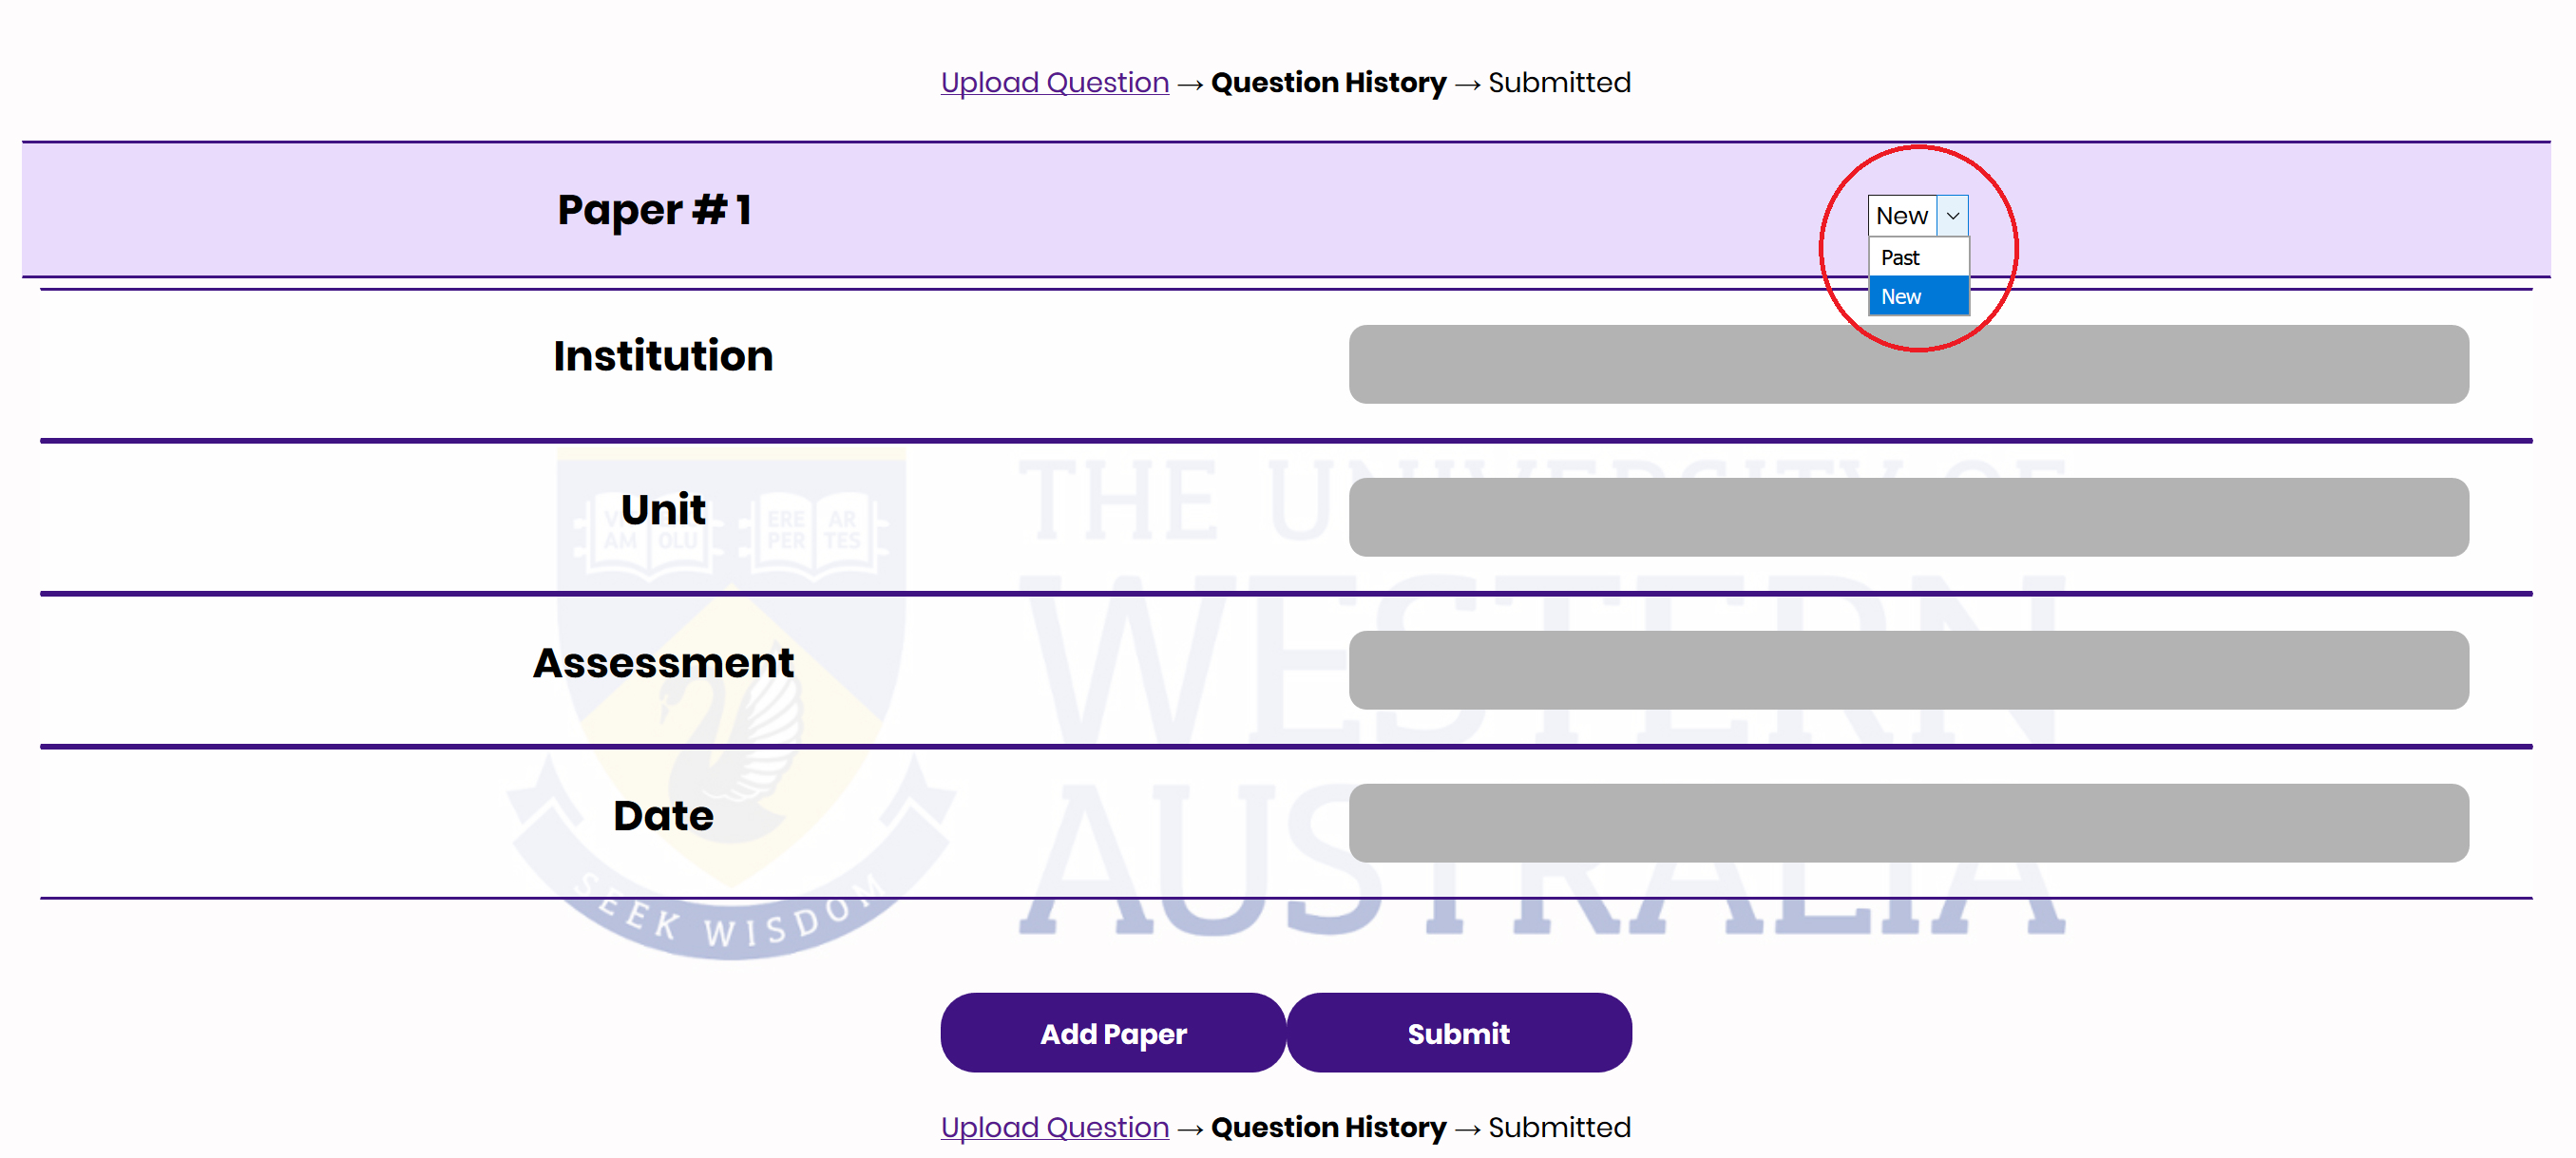
\includegraphics[width = 16cm, height = 8cm]{drop.png}
\caption{Selection Box to Choose between a Past or a New Paper}
\end{figure}
\pagebreak
\subsubsection{Picking a Past Paper}
After Selecting the ``Past Paper" option, you will be given a drop-down box of all prior papers associated with your account in the database\footnote{through creating tests through the application or through uploading other questions and selecting new paper}. Simply select one of these if the question was used in one. If the test you are looking for does not appear in this list, then you likely have not worked on that paper from this account, and should create a new paper.
\begin{figure}[H]
\centering
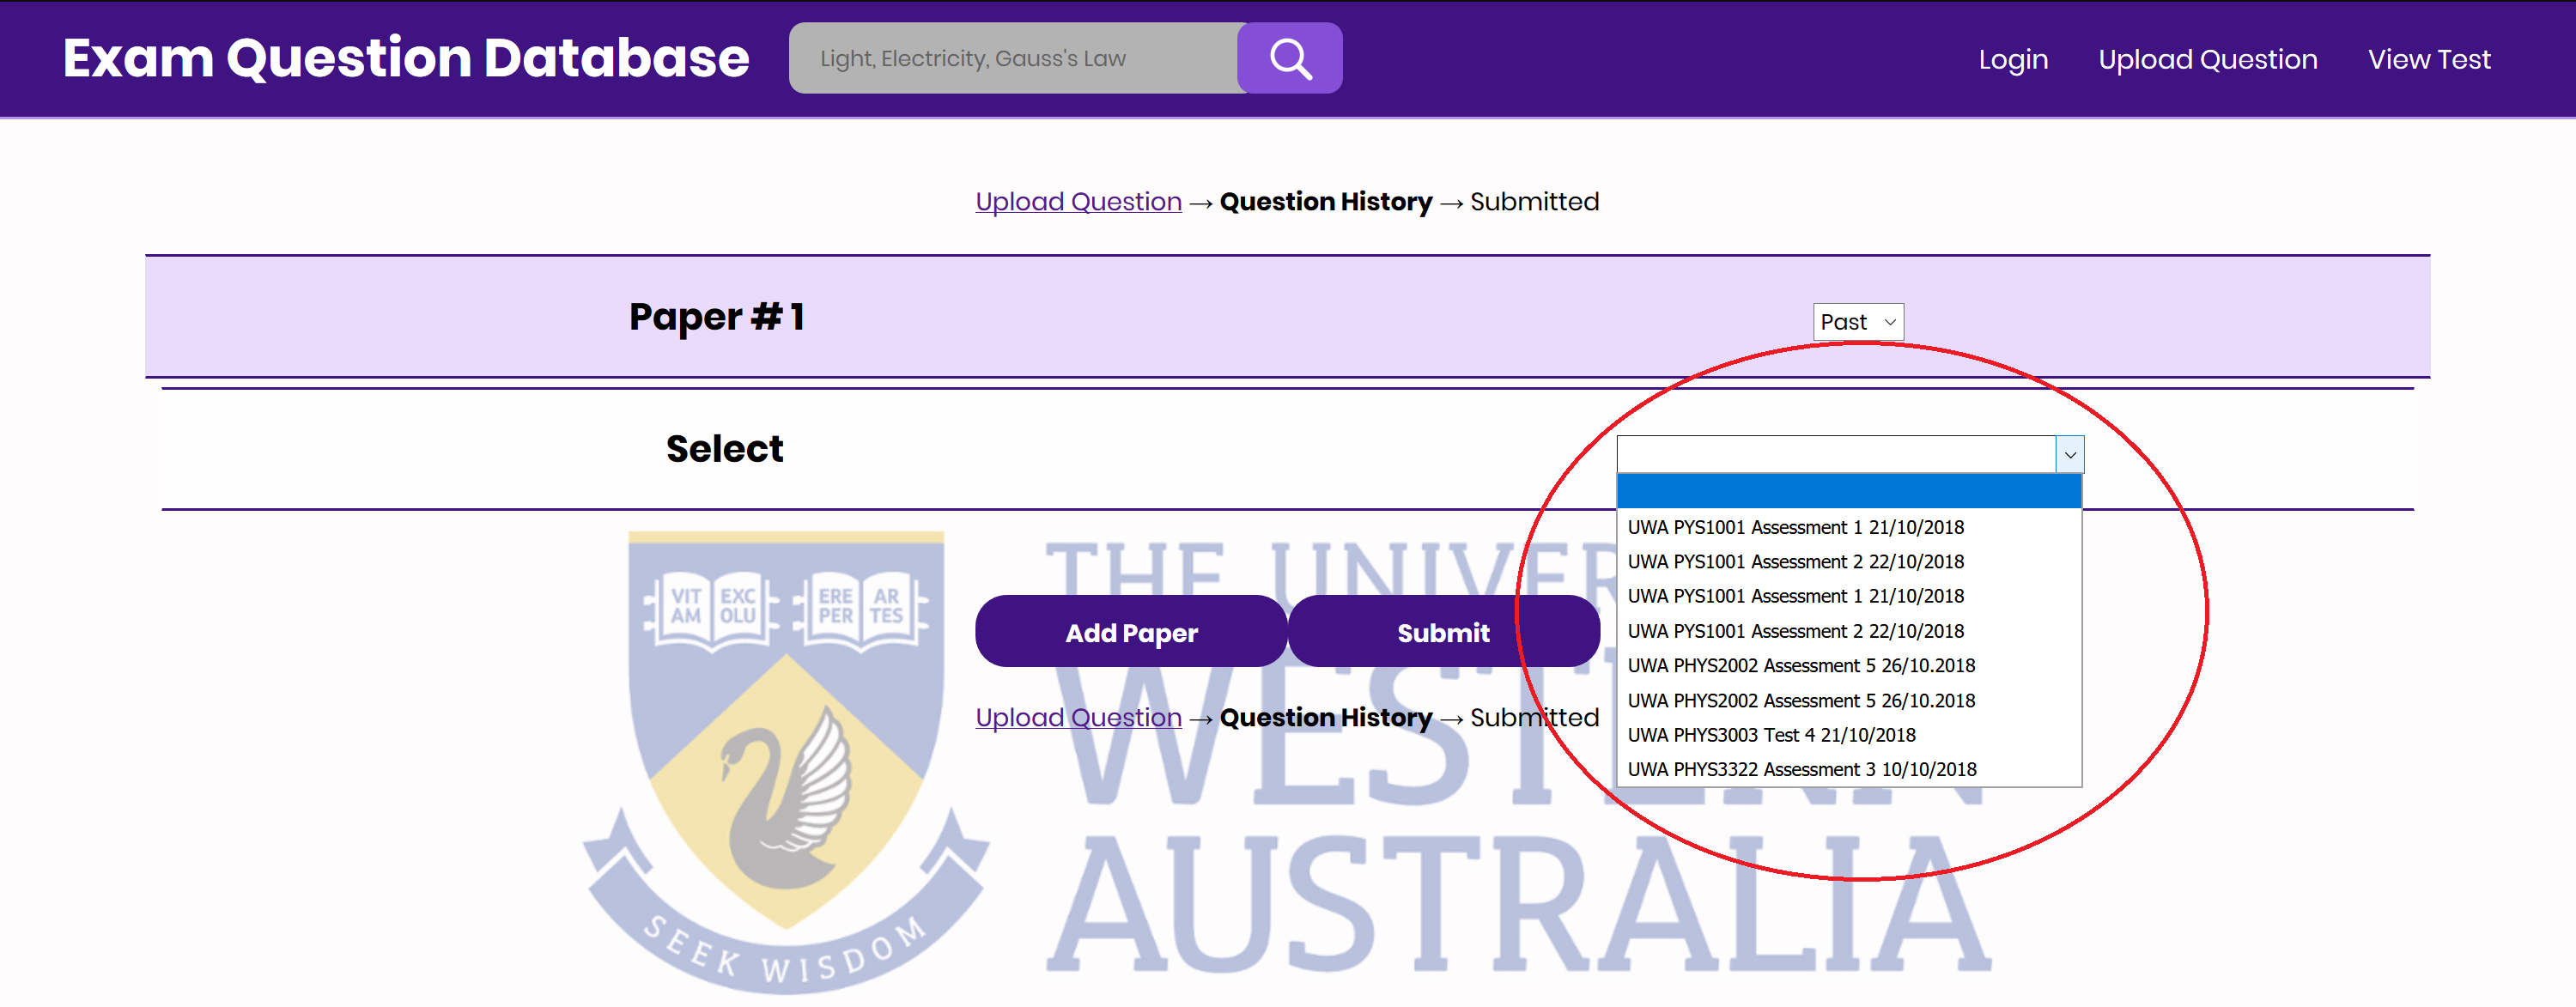
\includegraphics[width = 16cm, height = 7cm]{oldpaper.png}
\caption{Selection for Adding a Past Paper into a Question's History on Upload}
\end{figure}

\subsubsection{Adding a New Paper}
Selecting the ``New Paper" option will provide you with a series of text boxes in which you should state: The institution at which the question was used in this instance, the unit in which the question was used, the name of the assessment the question was used in, and the date of this assessment.
\begin{figure}[htp]
\centering
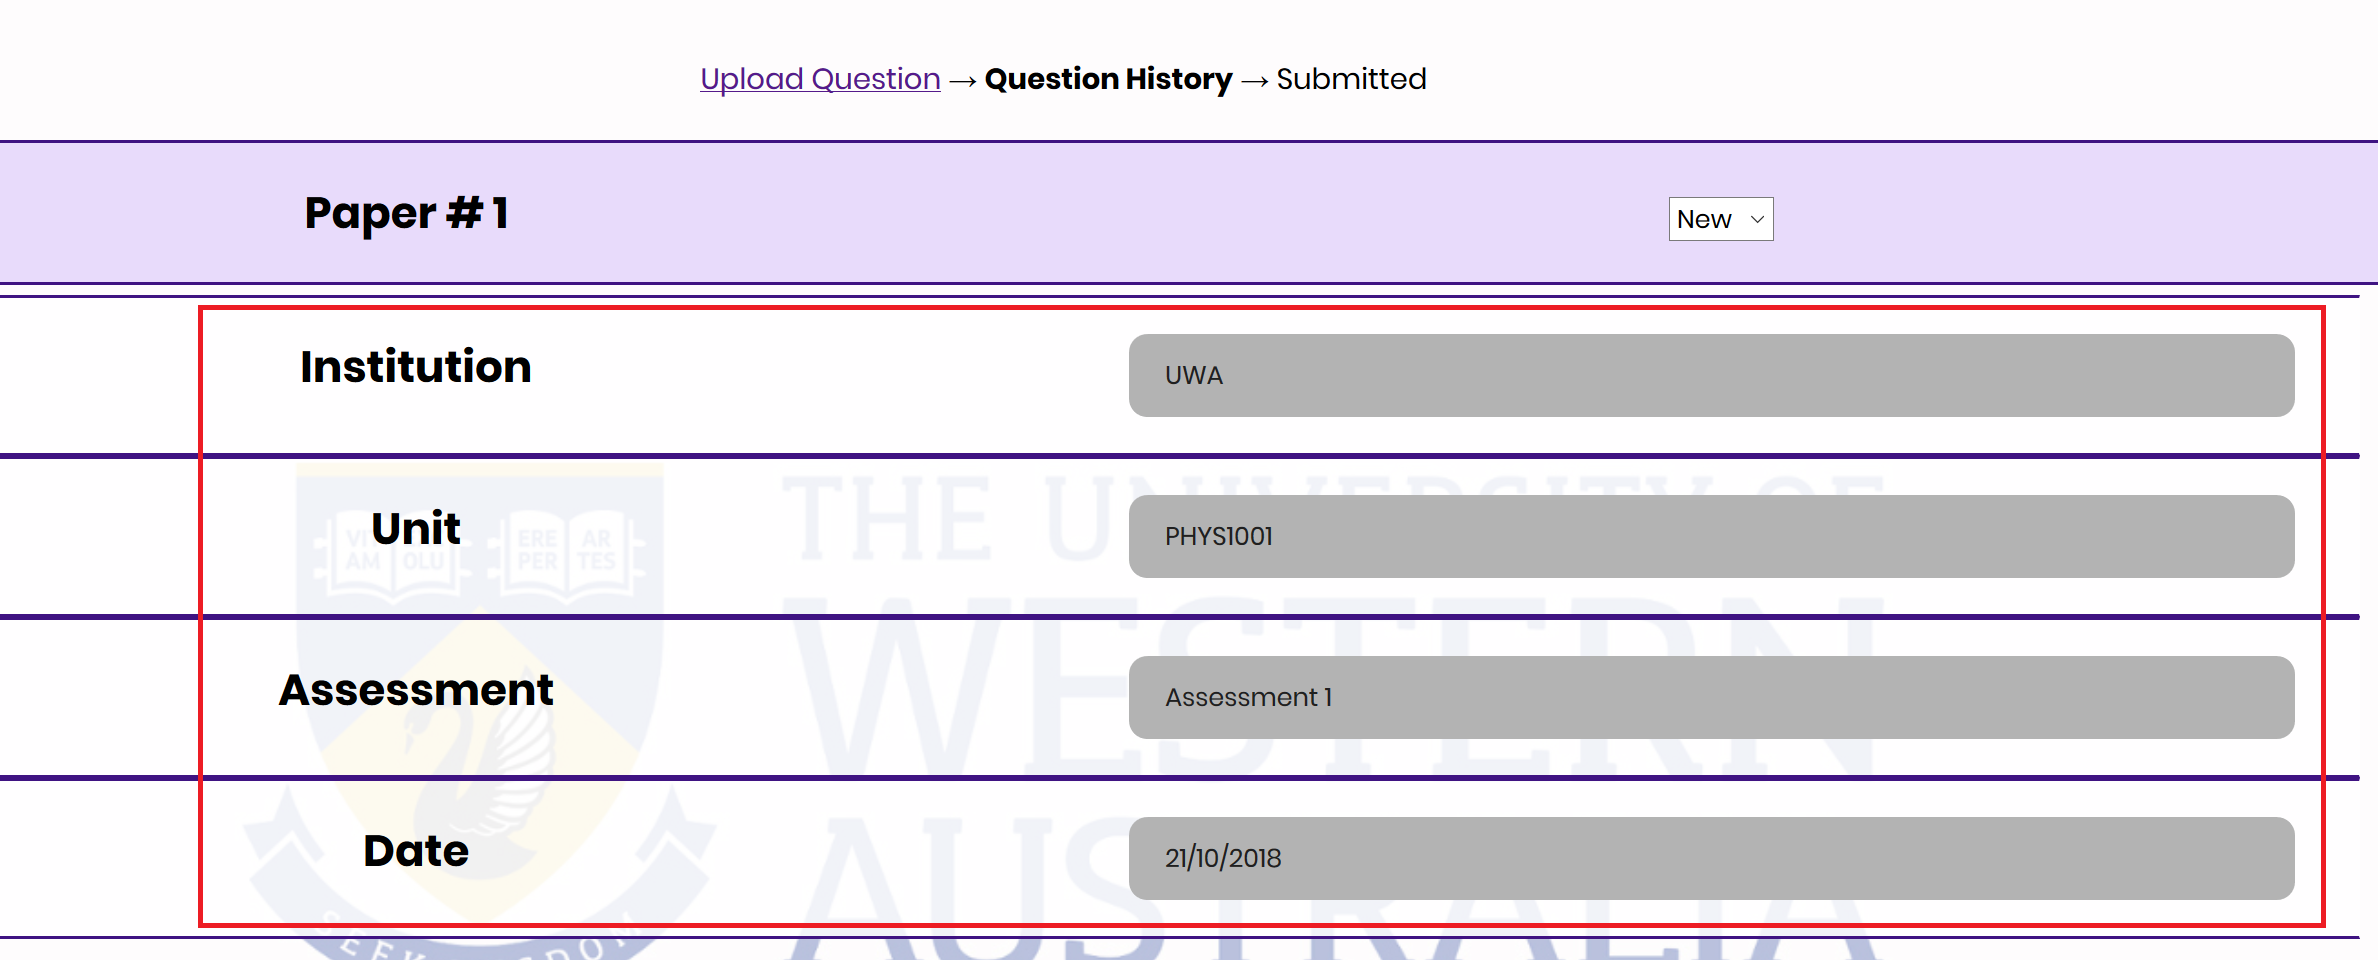
\includegraphics[width = 14cm, height = 7cm]{uphisv1.PNG}
\caption{Input Form for Adding a New Paper into a Question's History on Upload}
\end{figure}

\chapter{Adding Questions to a Paper} \label{ch:qadd}
\section{Searching the Database}
When using the application, once logged in, the homepage for the application is a search page you can use to search for questions by keyword. To search a question, click the grey text box and type any keywords you would like to search for questions relating to. Our system will then search the database for any questions related to these, and you will be redirected to a search results page. Alternatively, you may use the search bar included in the navigation bar of the page on any other page of the application.
\begin{figure}[htp]
\centering

\includegraphics[width =12cm]{SearchPage.PNG}
\caption{Search Bar on Application Search Page}
\end{figure}
\begin{figure}[htp]
\centering

\includegraphics[width =10cm]{PagetopSearch.PNG}
\caption{Navigation Bar Search Tool}
\end{figure}
\pagebreak
The results of your search will be displayed with a brief description of the contents of each question, the year in which each question was uploaded to the database, a link to a preview of each question, and a link to the previous usage history for that question.
\begin{figure}[H]
\centering
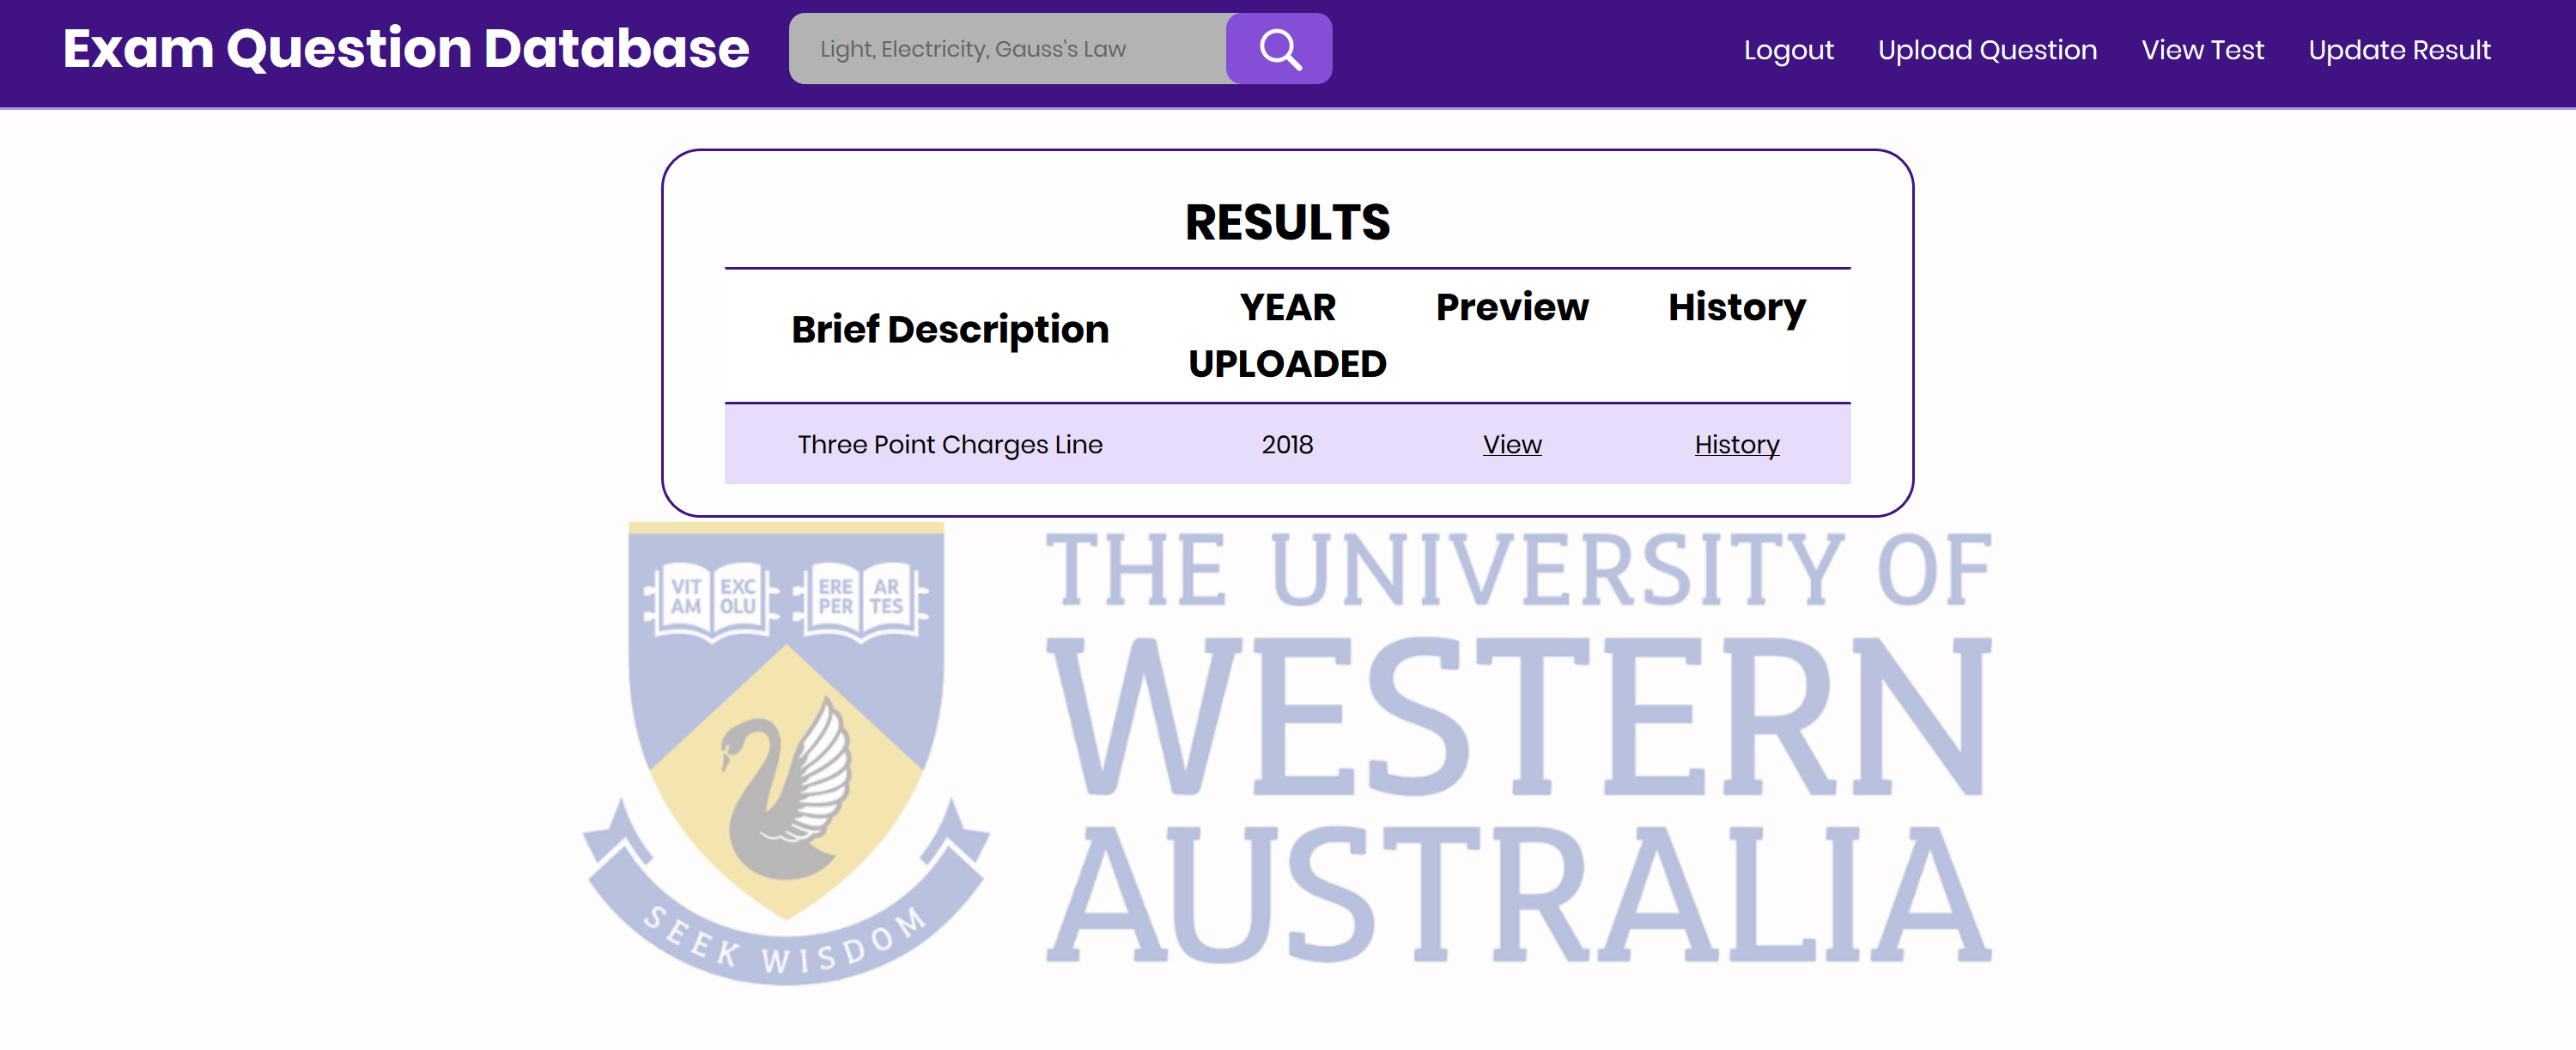
\includegraphics[width = 16cm, height = 8cm]{Result.PNG}
\caption{The Preview Page for an Example Question}
\end{figure}
\section{The History Page}
This page displays a row of information for each recorded occasion on which this question has been used for a formal assessment in the past. The columns in order show, for each assessment using the question, the institution which ran the assessment, the unit the assessment was a part of, the name of the assessment, the date of the use, and finally the result for this question in that assessment. The result is displayed as the number of students who correctly answered the question over the total number of students who sat the assessment.
\begin{figure}[H]
\centering
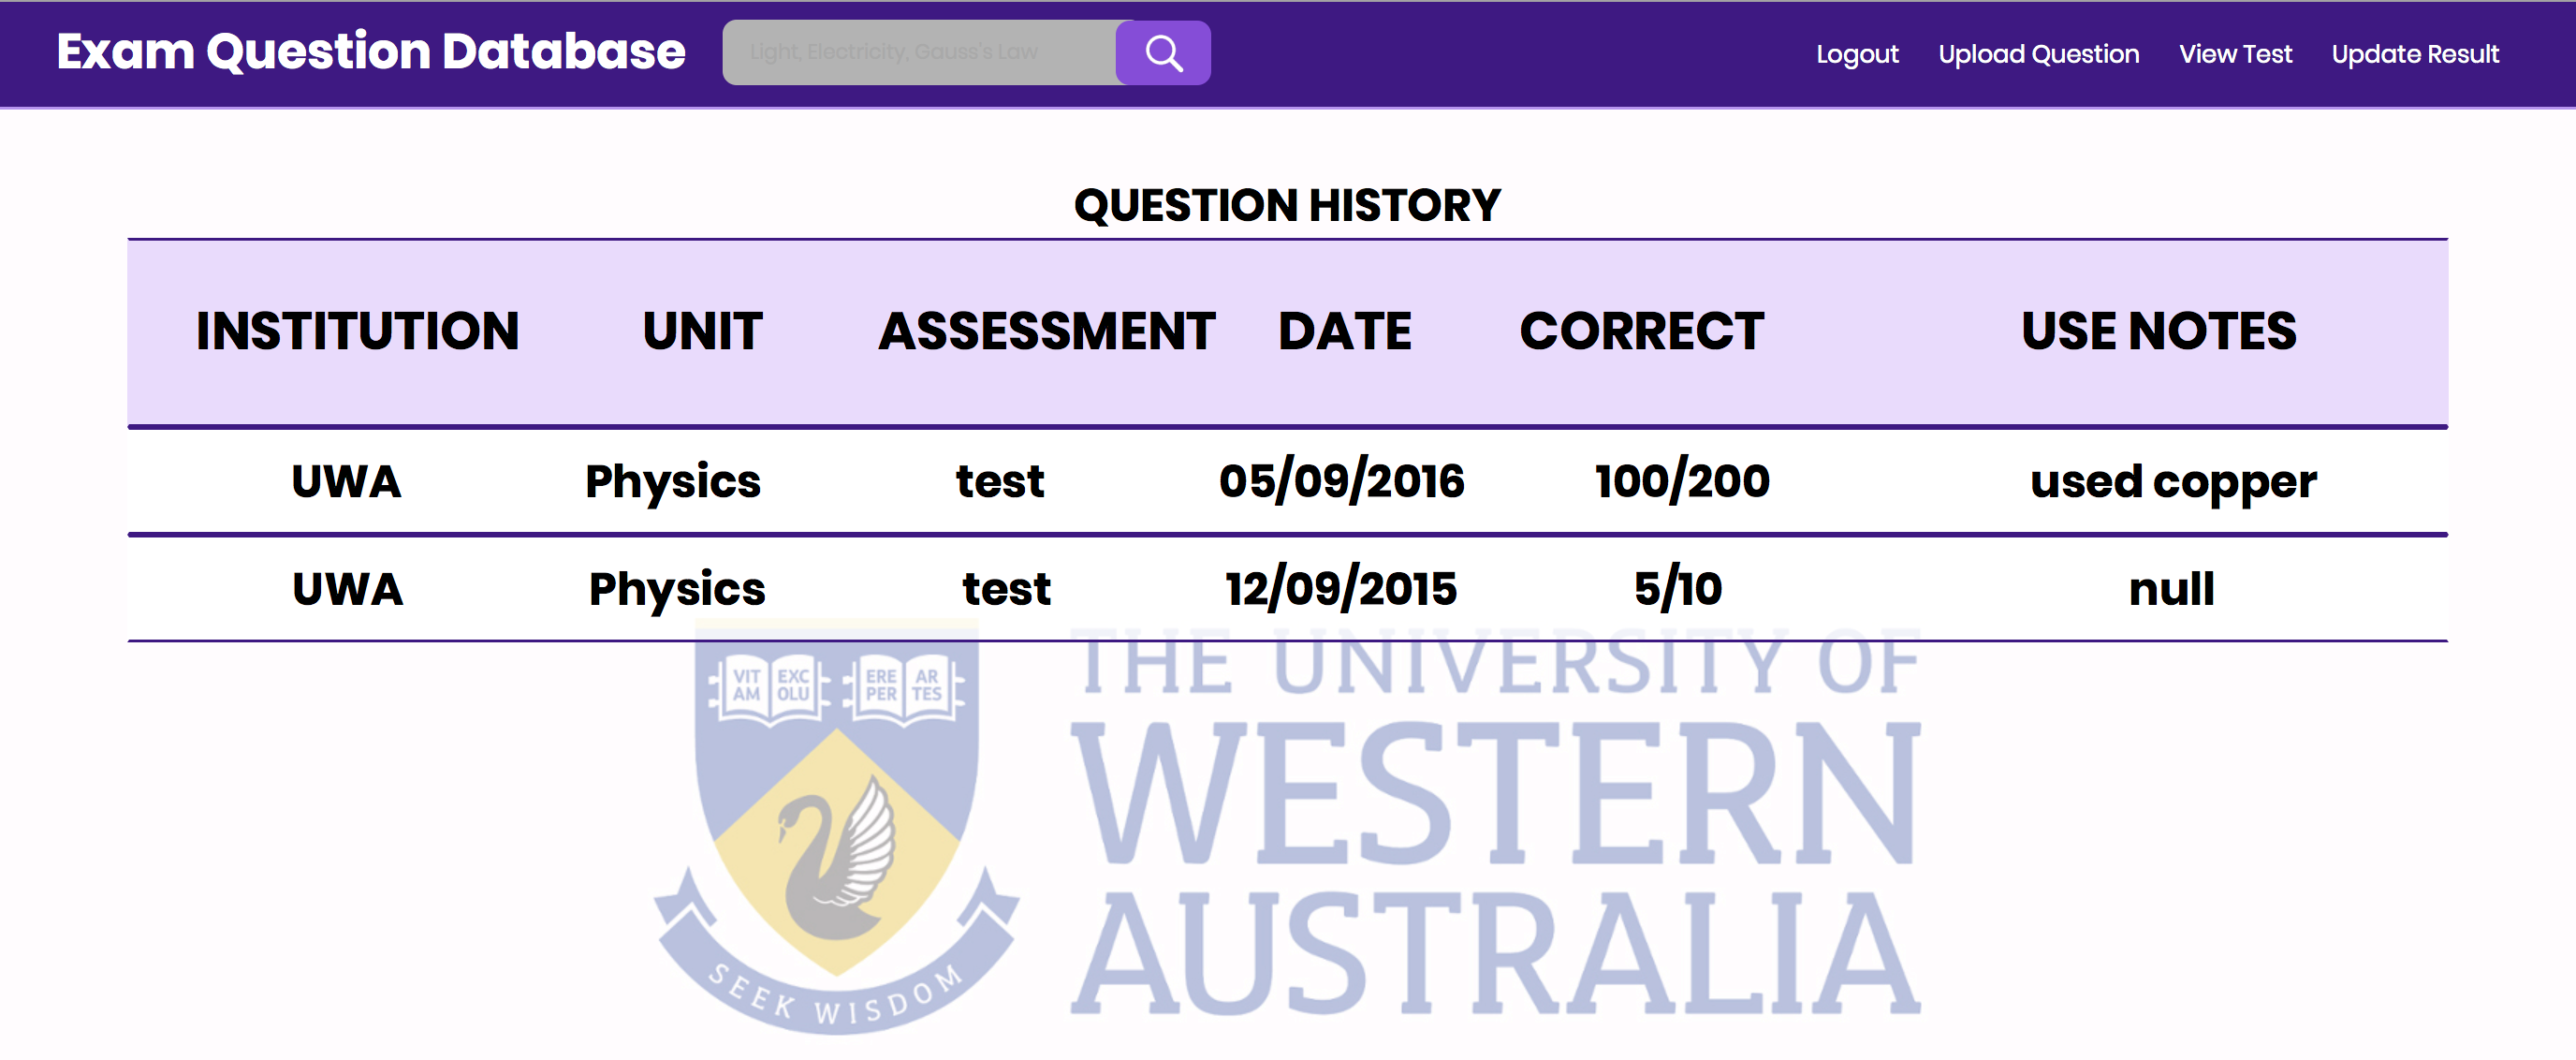
\includegraphics[width = 16cm]{HistoryPage.PNG}
\caption{The History Page for an Example Question}
\end{figure}
\pagebreak
\section{The Preview Page}\label{sec:pre}
This page shows what the question would look like as originally uploaded to the database, to give you an idea of any graphics included and show the question beying just the brief description.\par
This page is also the page from which you can choose to add a question to your currently in progress test by clicking on the Add to Test button (1), although if your test includes this question already, button (1) will be inactive. You can also choose to view the question's use history from this page by clicking on the History button (2). Once you click to add a question to a test you will be redirected to a confirmation of this action, and you can again search for more questions.\footnote{the topic and subtopic fields have since this screenshot been changed to key-words}
\begin{figure}[H]
\centering
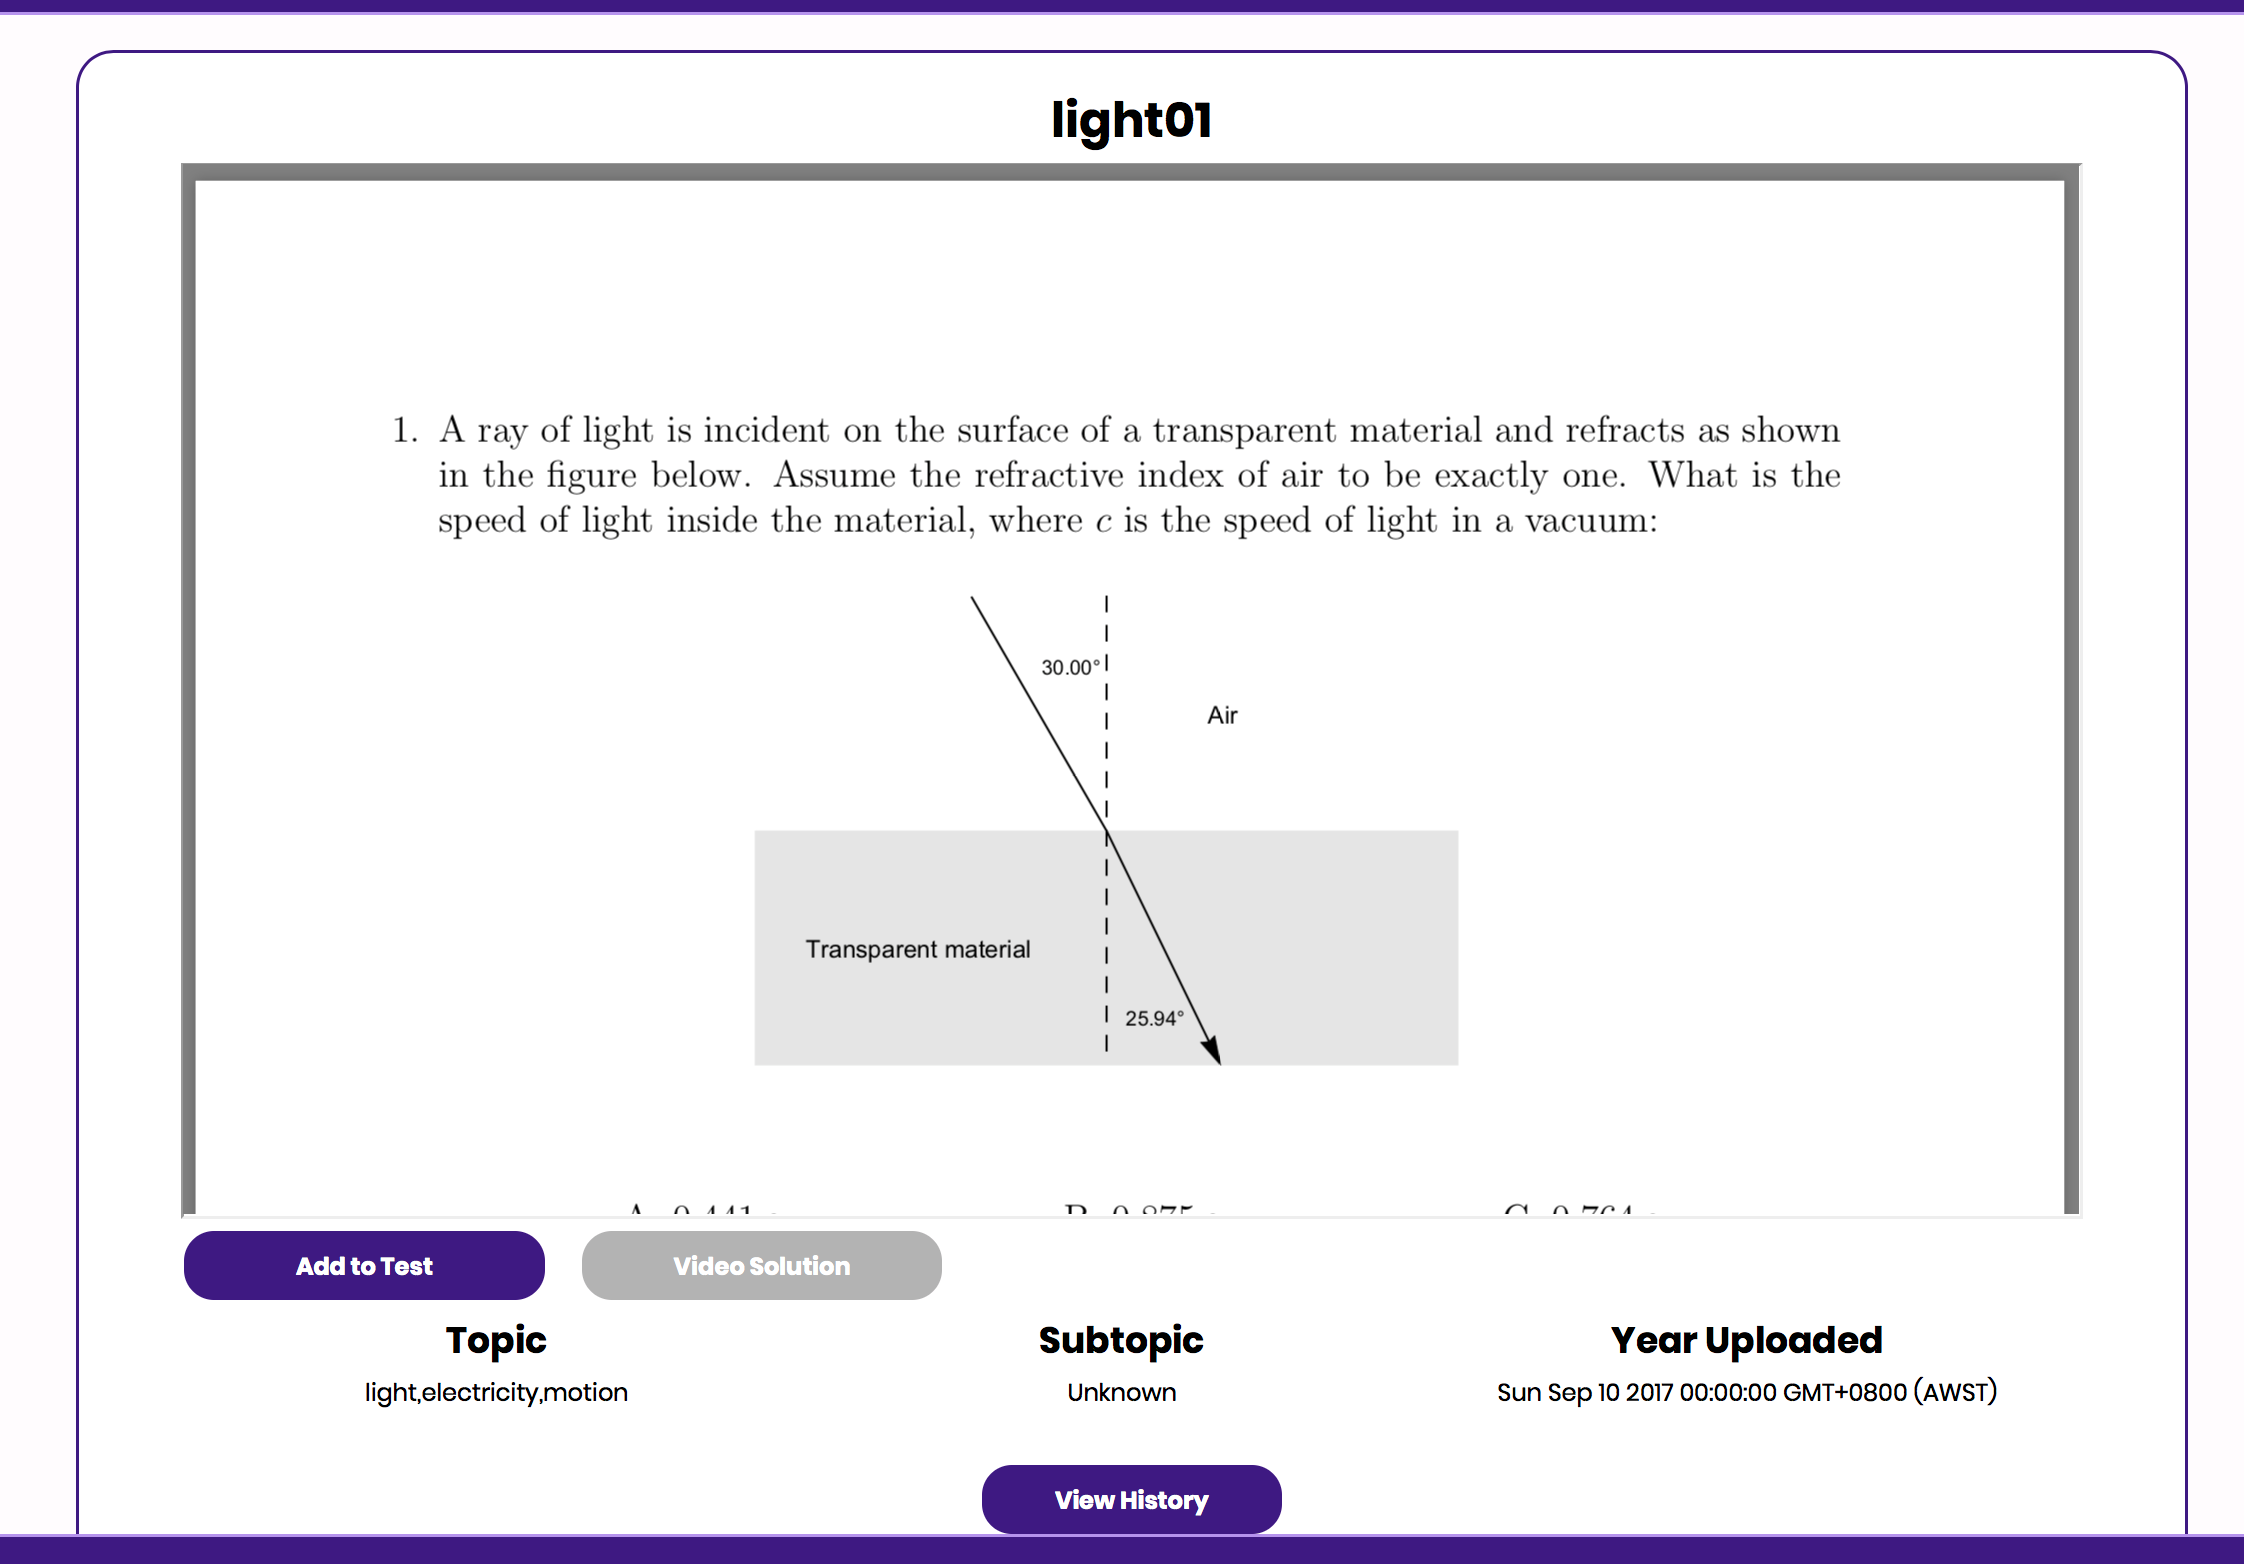
\includegraphics[width = 16cm, height = 15cm]{preview.png}
\caption{The Preview Page for an Example Question*}
\end{figure}


\chapter{Viewing Contents and Downloading a Paper}
\section{Viewing the Contents of a Paper}
To view the contents of a paper currently being worked on, you need to click ``View Test" in the navigation bar, this will redirect you to a page displaying the current questions within your current paper, and will allow you remove these by clicking the red (X) buttons beside the question you wish to remove. You can find any question you accidentally remove by searching again for the question (as per chapter \ref{ch:qadd}). In this page there is also a link to the preview of each question, as discussed in section \ref{sec:pre}.\par
\begin{figure}[H]
\centering
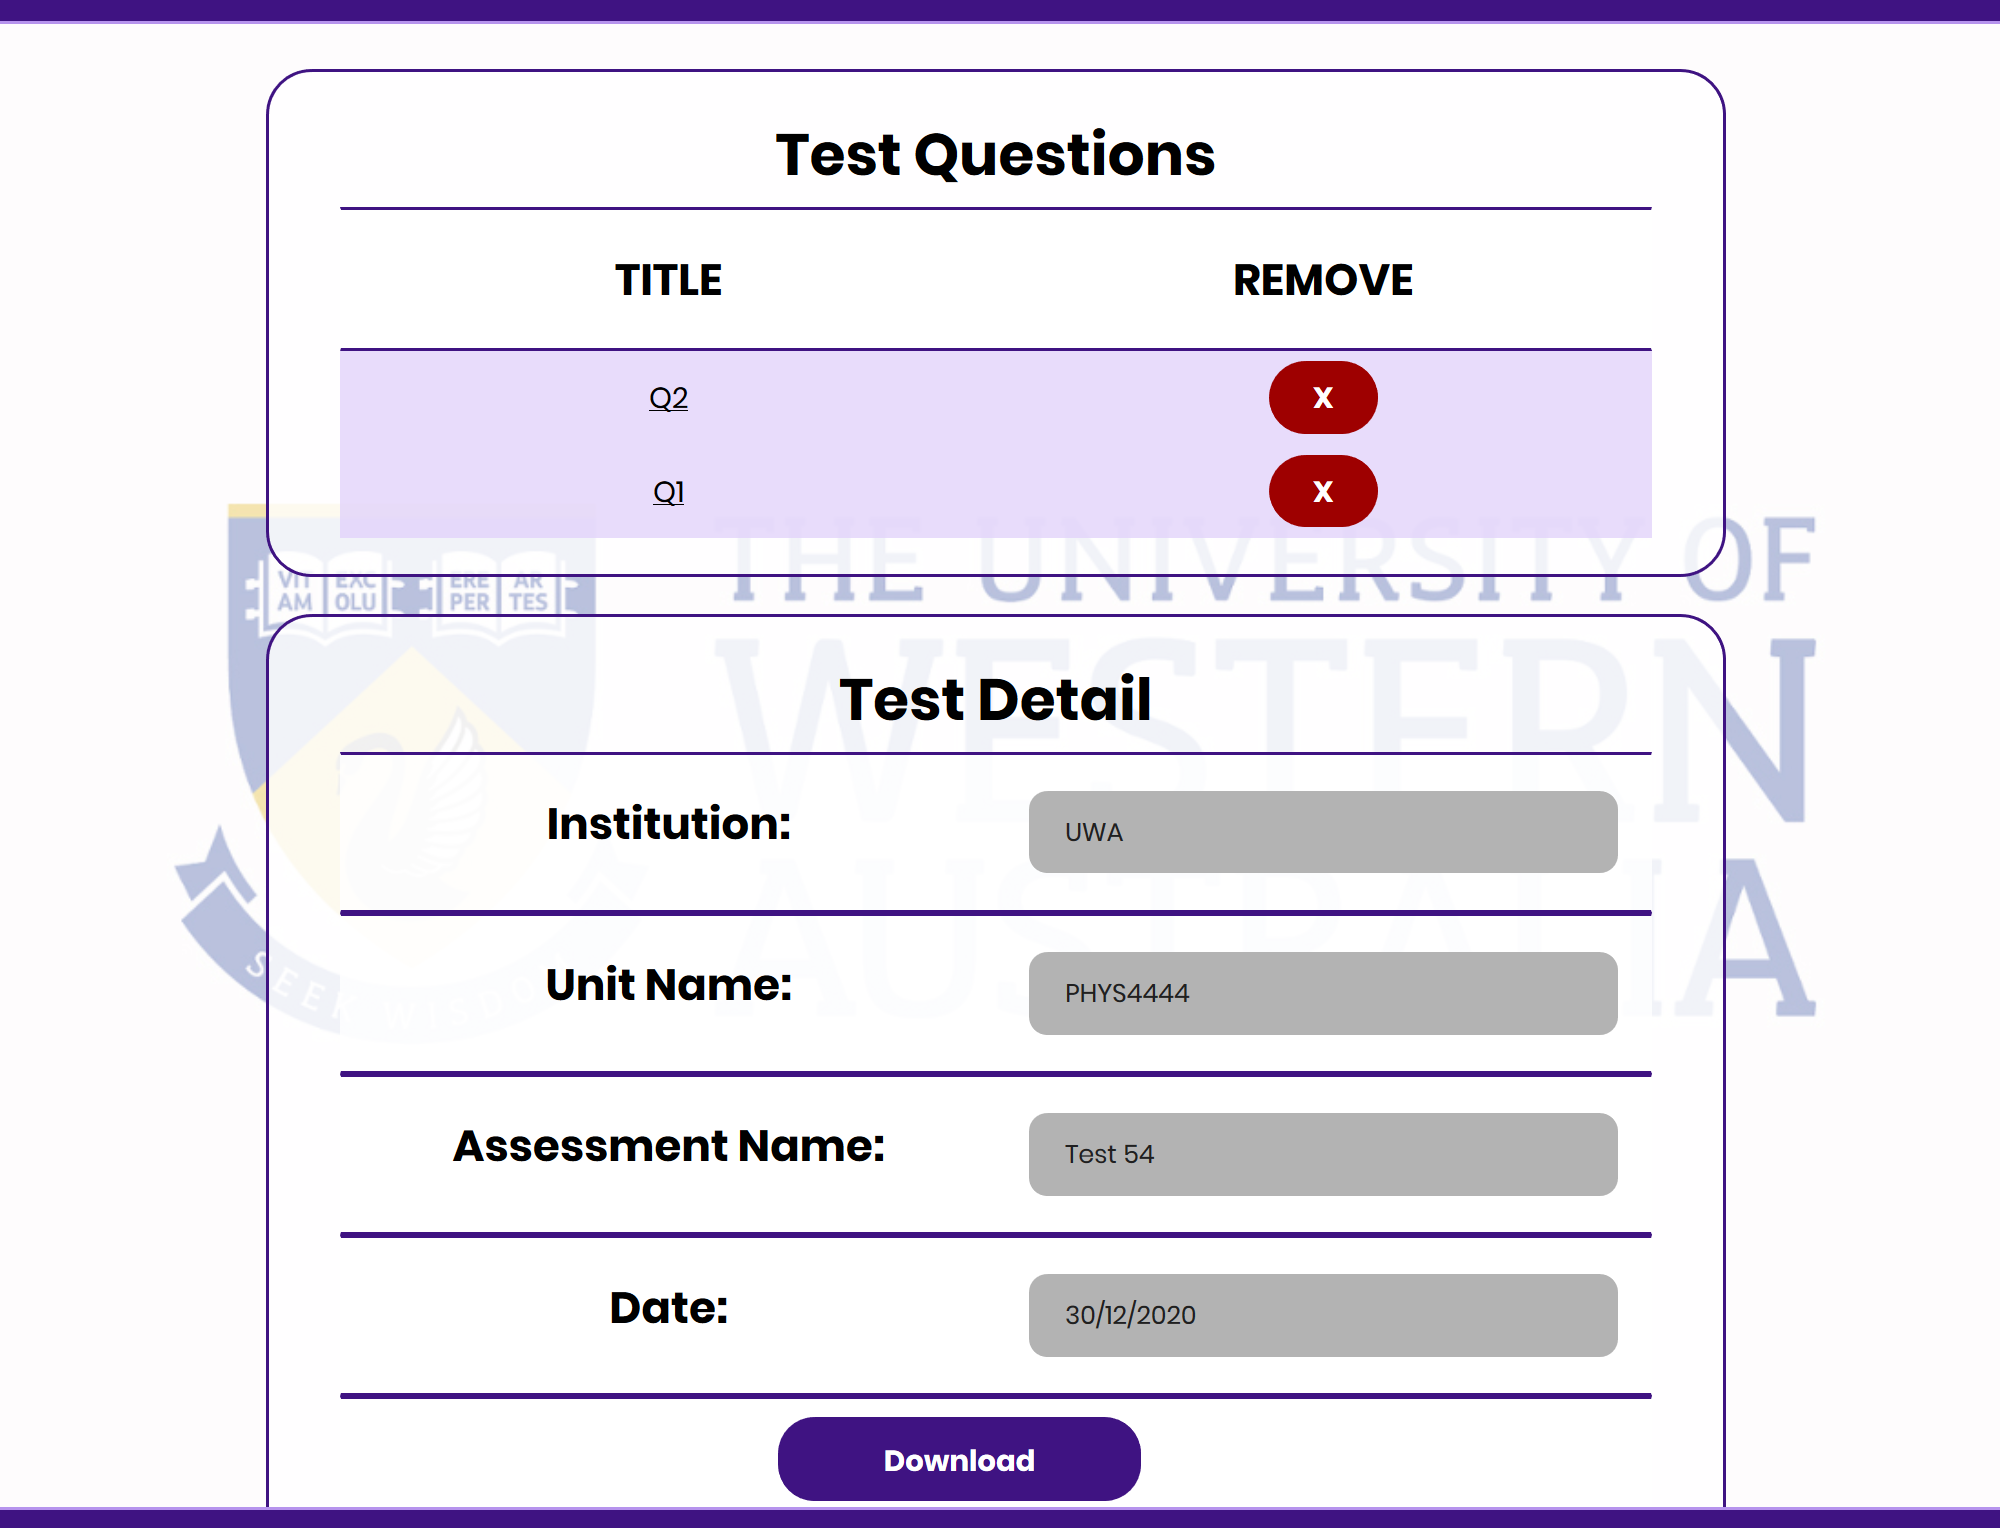
\includegraphics[height = 12cm]{viewtest.png}
\caption{The View In Progress Test Page}
\end{figure}

\section{Downloading a Paper}
To download a paper, simply click the "Download" button at the bottom of the page. \par You will receive a compressed (.ZIP) folder containing a .tex file containing the files for each question appended together, and a sub-directory called 'figs' containing the images from each question.
\par \textbf{Note: Figure references in the combined test file may not match 1:1 with images in the figs folder, and some file names and paths may need changing in the .tex file or the figs folder manually.}
\subsection{Paper Information}
To download a paper you first need to give information about the paper. To do this you need to fill in the information on the contents and download page. 	There are four fields which need to be filled in for each paper to uniquely identify it:
\small
\par -The first field you need to fill in is the \textbf{Institution }at which the paper is being used \par (e.g. UWA, ANU)
\par -The second field is the \textbf{Unit} in which you are using the paper (e.g. PHYS1001, CITS3200)
\par -The third field is the \textbf{Assessment} name (e.g. Test: Optics, Exam, Assignment 3, Test 2)
\par -Finally you should input the \textbf{Date} that the assessment will run. \textbf{Use the DD/MM/YYYY} \par \textbf{as suggested by the input field when blank.}
\normalsize
\\ When all fields are filled in, \textbf{and you are sure you're ready to download this paper}\footnote{Even you click cancel after clicking the download button you will create this paper in the database still and the cart will empty}, click the download button.
\begin{figure}[H]
\centering
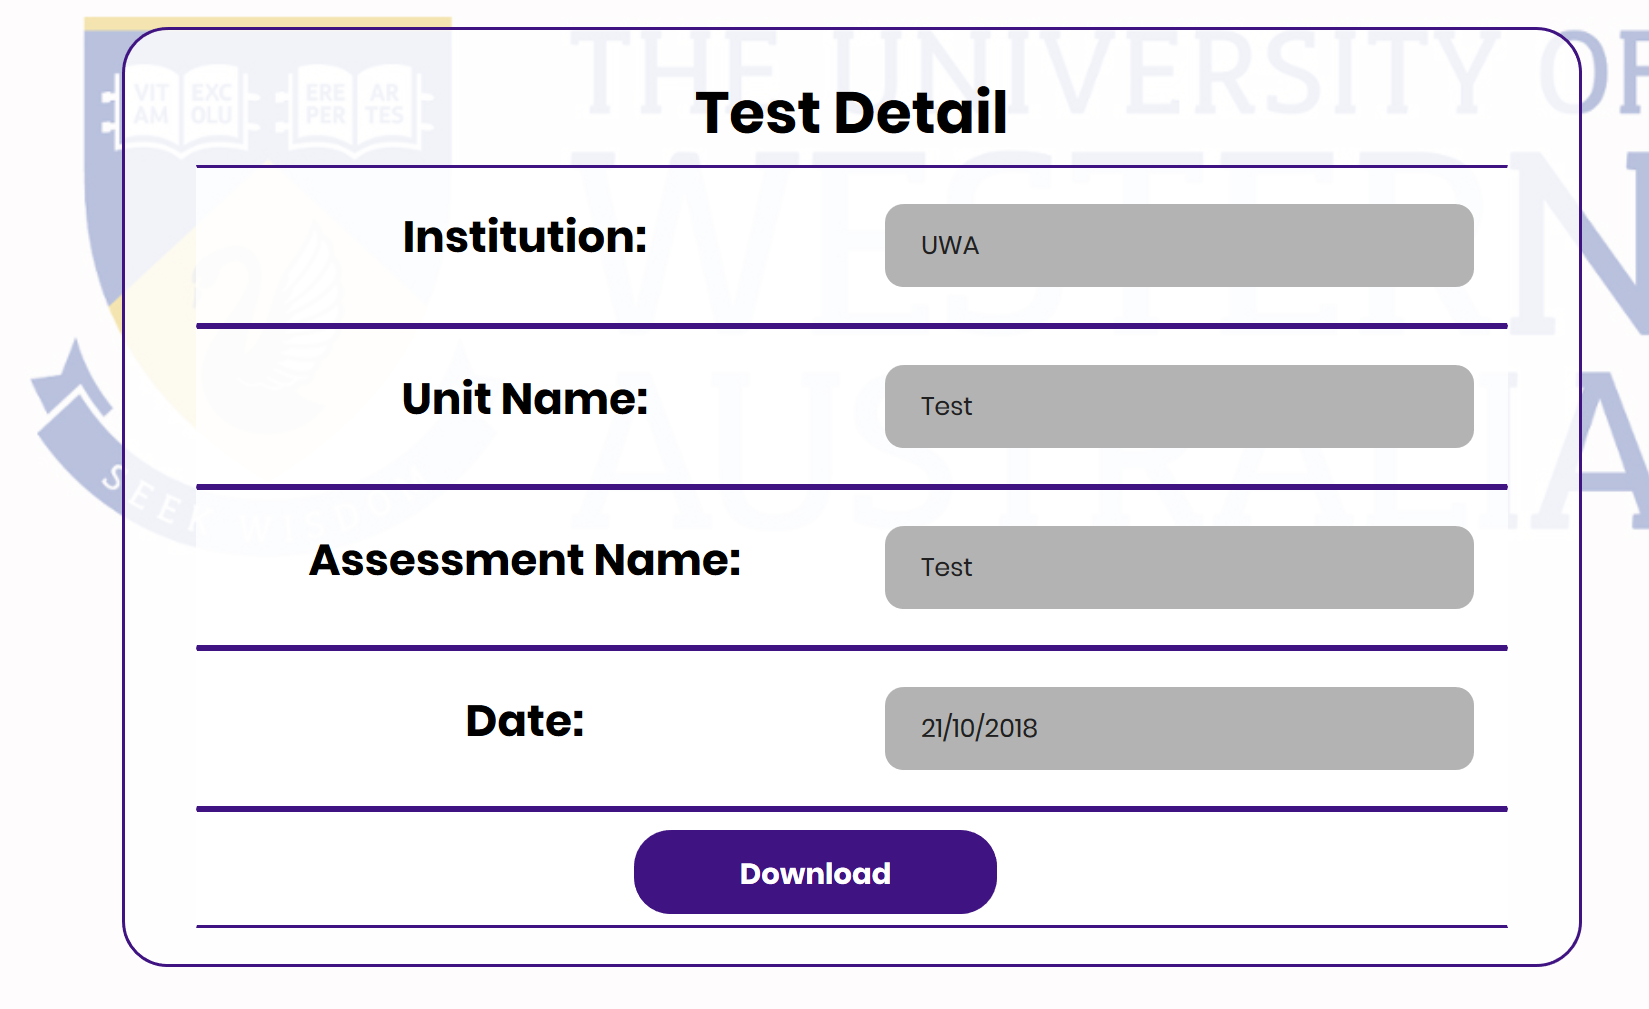
\includegraphics[height = 9cm]{Downloads.PNG}
\caption{The Form for Downloading a Paper}
\end{figure}



\chapter{Updating a Paper's Results}\label{ch:upres}
\section{Viewing Your List of Past Papers}
To access a list of all the papers you have worked on in the past you can click on ``Update Result'' in the navigation bar, this will redirect you to a page containing a list of all the papers you have worked on in the past.\par To go to the page to update the results of a paper, simply click on a paper, and you will be taken to the page for that paper.
\begin{figure}[htp]
\centering

\includegraphics[width =16cm]{NavBarPapRes}
\caption{Navigation Bar with ``Update Result'' Circled}
\end{figure}
\begin{figure}[H]
\centering
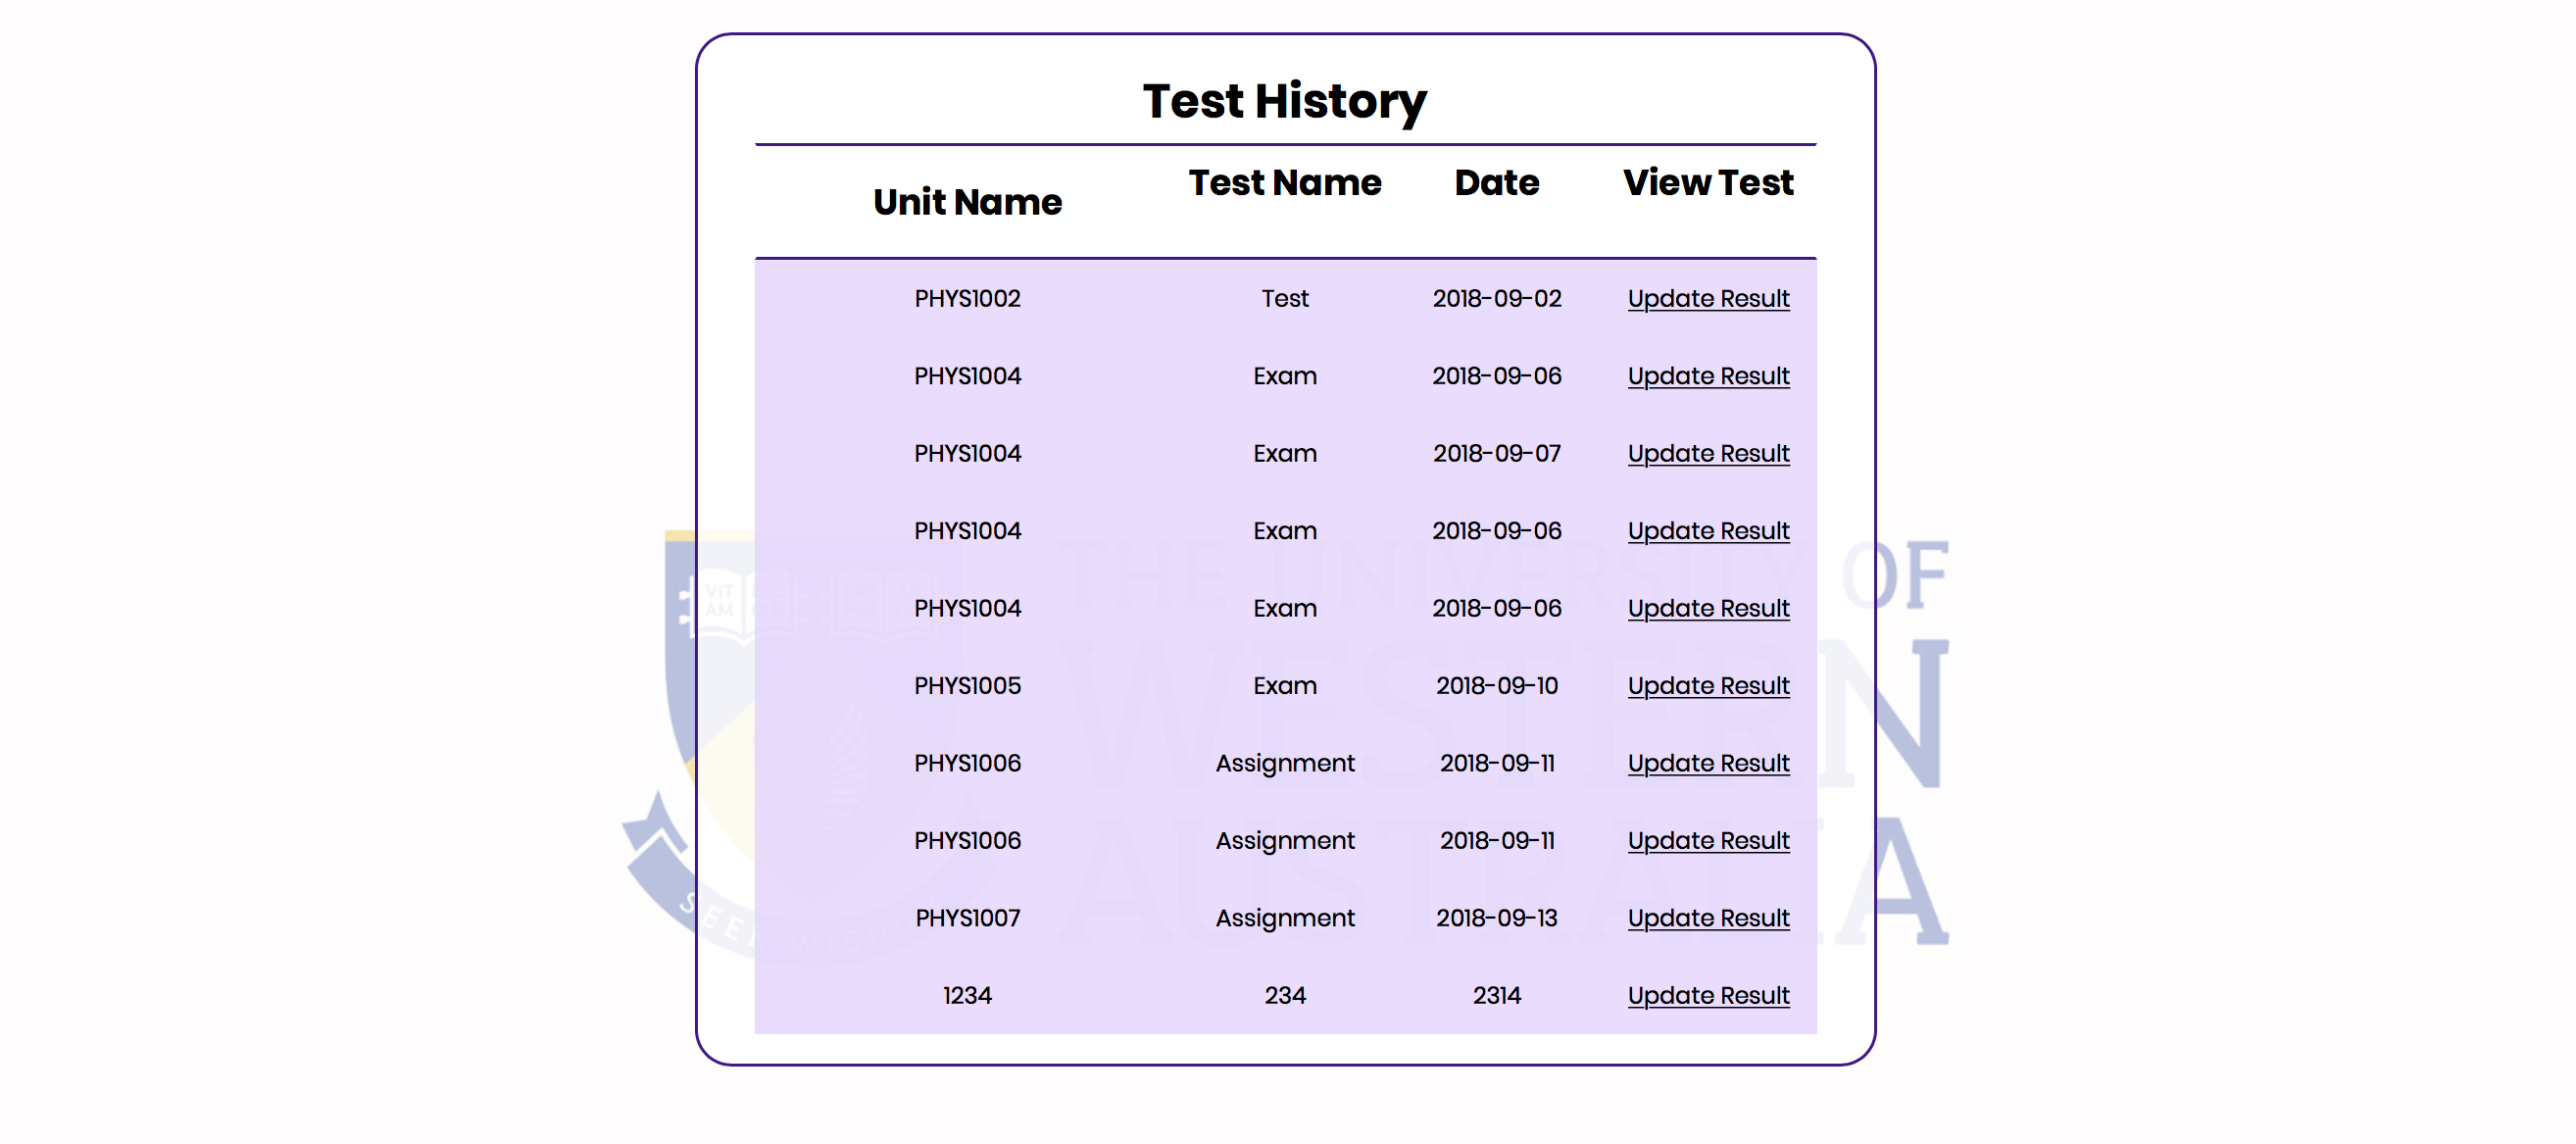
\includegraphics[width = 16cm]{testhistory.png}
\caption{Page Containing All of a User's Past Papers}
\end{figure}
\pagebreak
\section{Updating the Results for a Paper}
Once on the page for a single paper, you will see each question laid out in order. For each question, a brief description will be shown and you will be able to see a preview (as in section \ref{sec:pre}).
\\There will then be \textbf{three} input fields relating to each question:
\par -The first of these is where you may put any notes about \emph{variation }in the form of the question from that in the database in this paper.
\par -The second of these is the space for you to enter the \textbf{number} of sudents who answered the question correctly.
\par -The third of these spaces is for you to enter the total \textbf{number }of students who answered this question.

\begin{figure}[H]
\centering
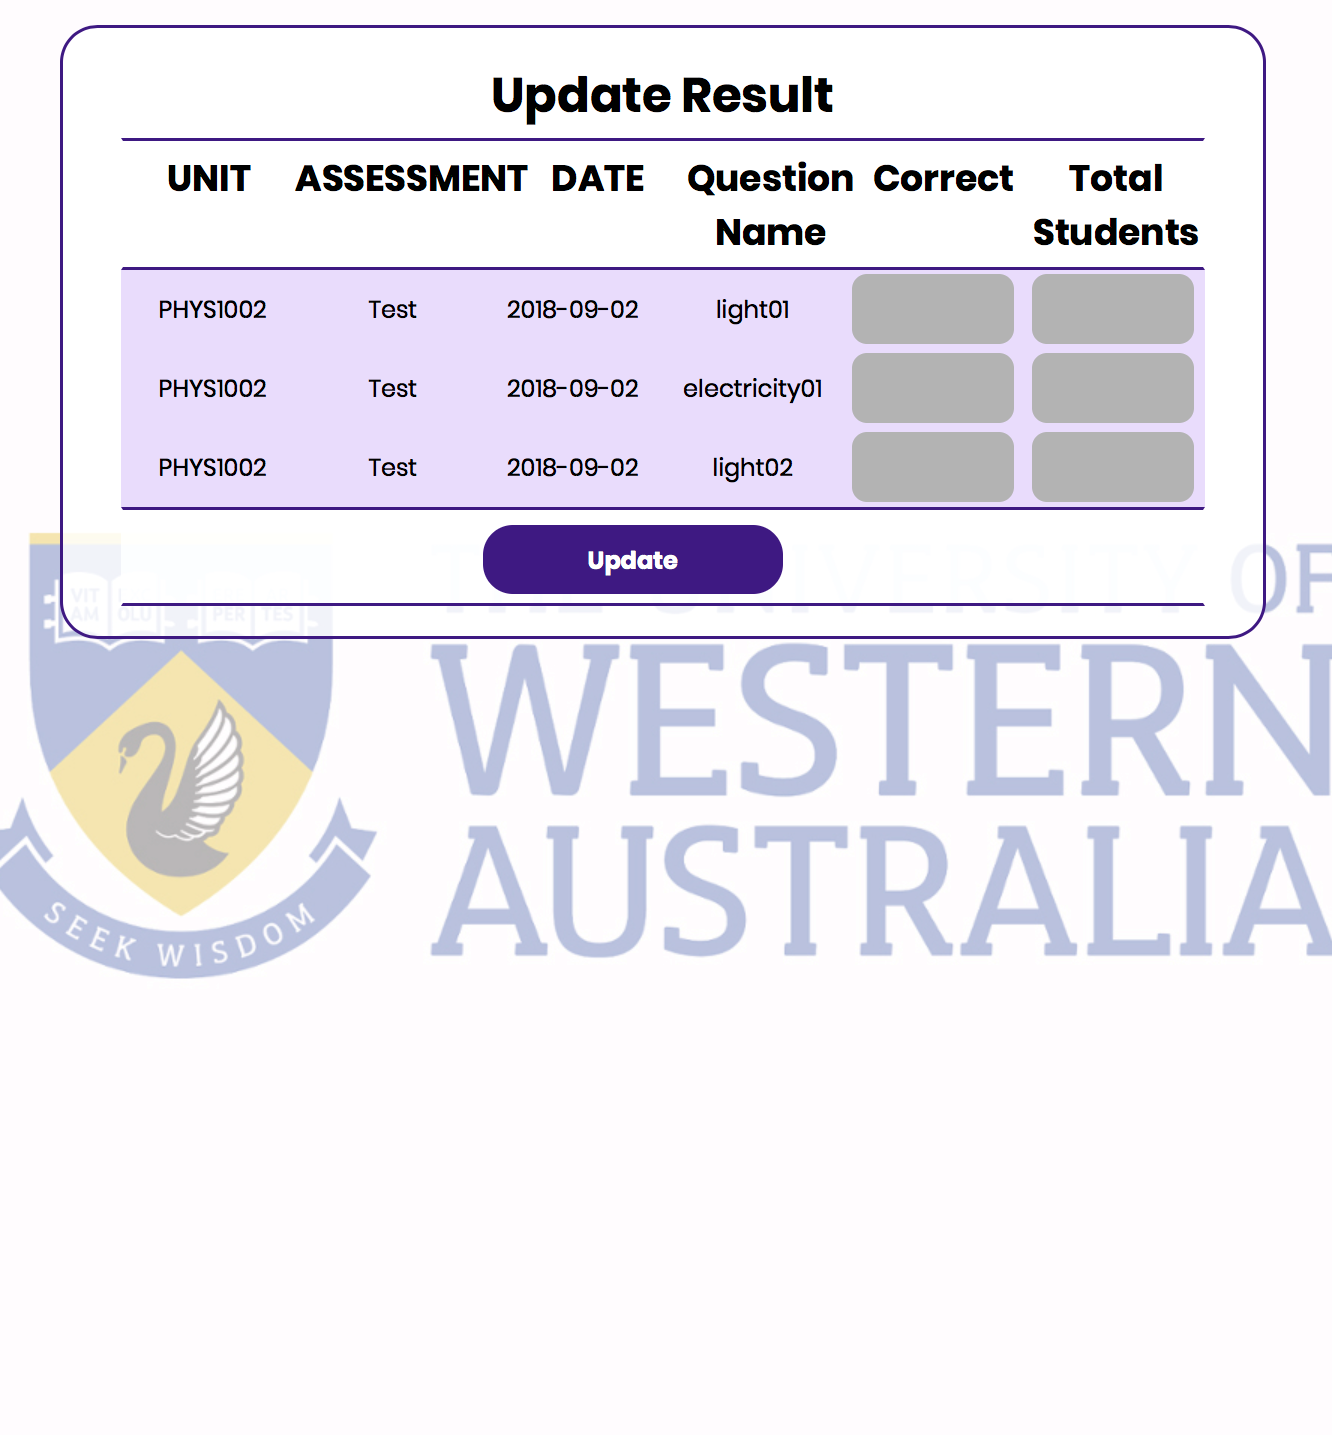
\includegraphics[width = 12cm, height = 15cm]{Updateresults.png}
\caption{The Preview Page for an Example Question}
\end{figure}
\begin{appendices}
\addappheadtotoc

\chapter{A Notice About User Deletion}
\small
The database behind this system is a MySQL Relational Datanase in which changes in some tables are cascaded throughout the database. More specifically: when there an entry in a table gets updated or deleted, \emph{associated entries in other tables will be affected similarly}. Specifically one should be careful when deleting users, as this may cause all data associated with this user to be removed from the database, \textbf{including any questions uploaded to the database by this user}.
\\
\par An Example Follows:
\begin{figure}[H]
\centering \subfloat[Original User Table]{{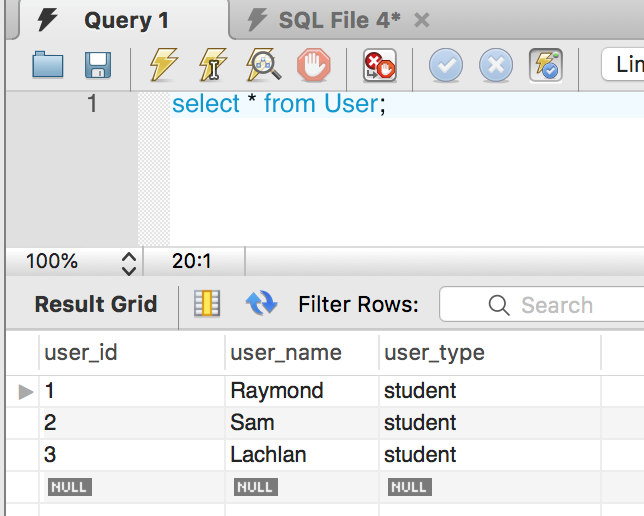
\includegraphics[width=4cm, height = 6cm]{origusetable.PNG} }}%
    \qquad
    \subfloat[Original Paper Table]{{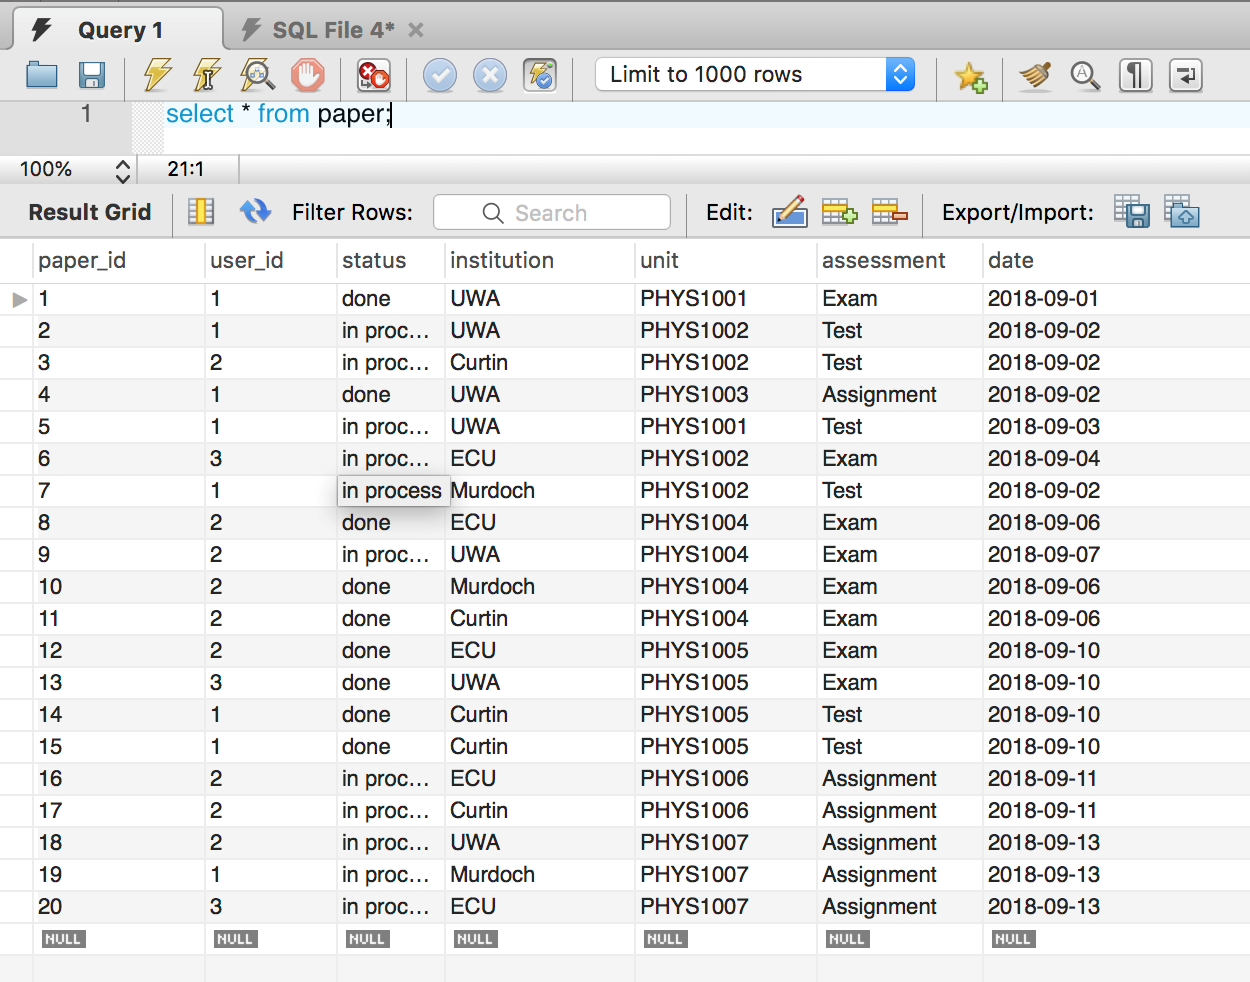
\includegraphics[width=5cm, height =6cm]{origpaptable.PNG} }}%
    \qquad
    \subfloat[Original In-Progress Papers Table]{{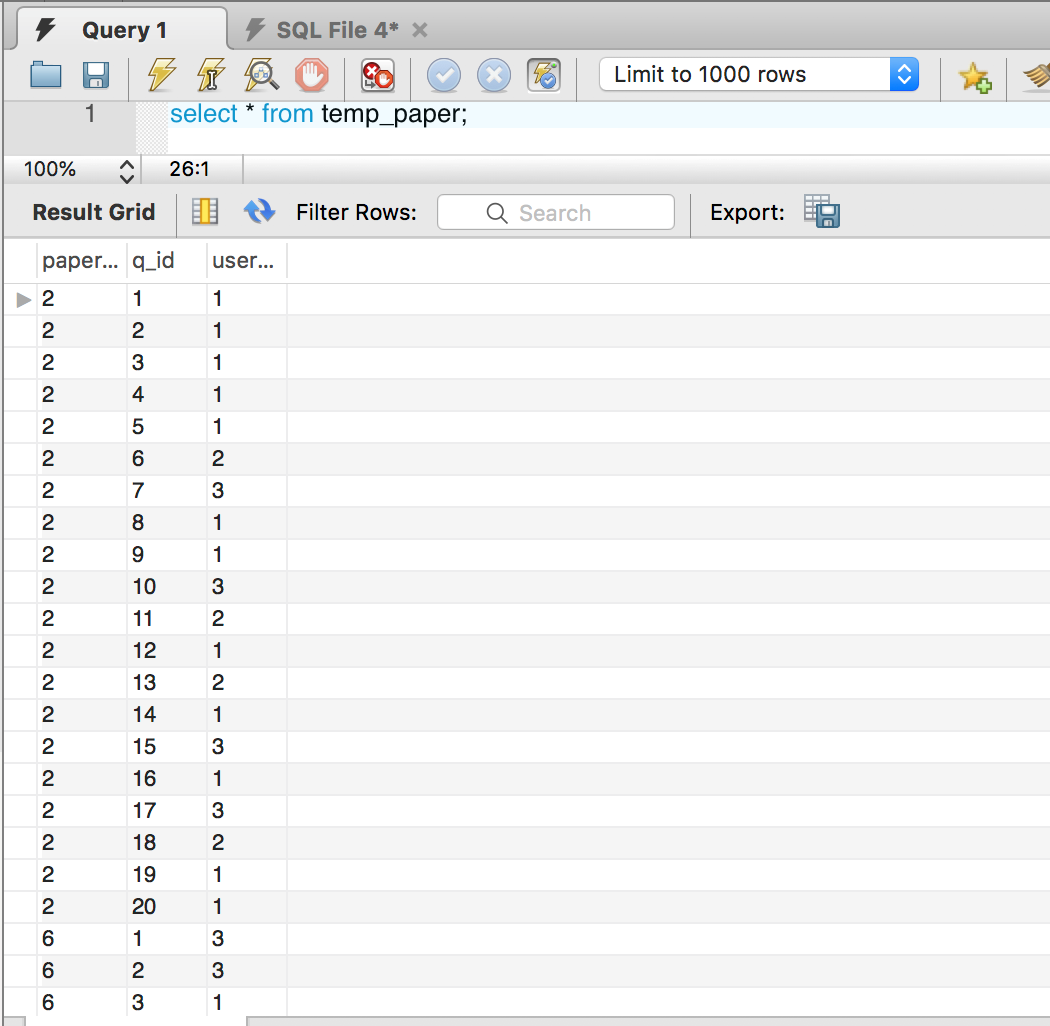
\includegraphics[width=5cm, height = 6cm]{origtemptable.PNG} }}%
    \caption{Tables Prior to the Delete User Query}%
    \label{fig:DBpredel}%
    \end{figure}
 \par Now, deleting the user with id = 2:
\begin{figure}[htp]
\centering
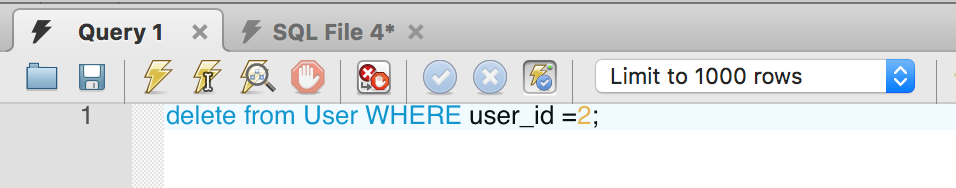
\includegraphics[width = 8cm, height = 2cm]{delquer.png}
\caption{Deletion Query for User Where UserId = 2}
\end{figure}\pagebreak
\par We end up with the new user table
\begin{figure}[H]
\centering
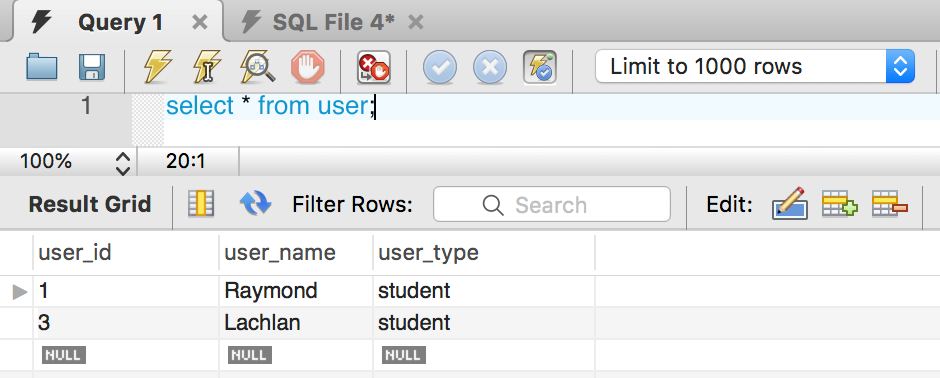
\includegraphics[width = 10cm, height = 3cm]{newusetable.png}
\caption{User Table from fig \ref{fig:DBpredel} After the Deletion Query}
\end{figure}
\par However we can also see that all records with reference to User Id = 2 in Paper and Temp\_Paper are also removed:
\begin{figure}[H]
\centering
\subfloat[New Paper Table]{{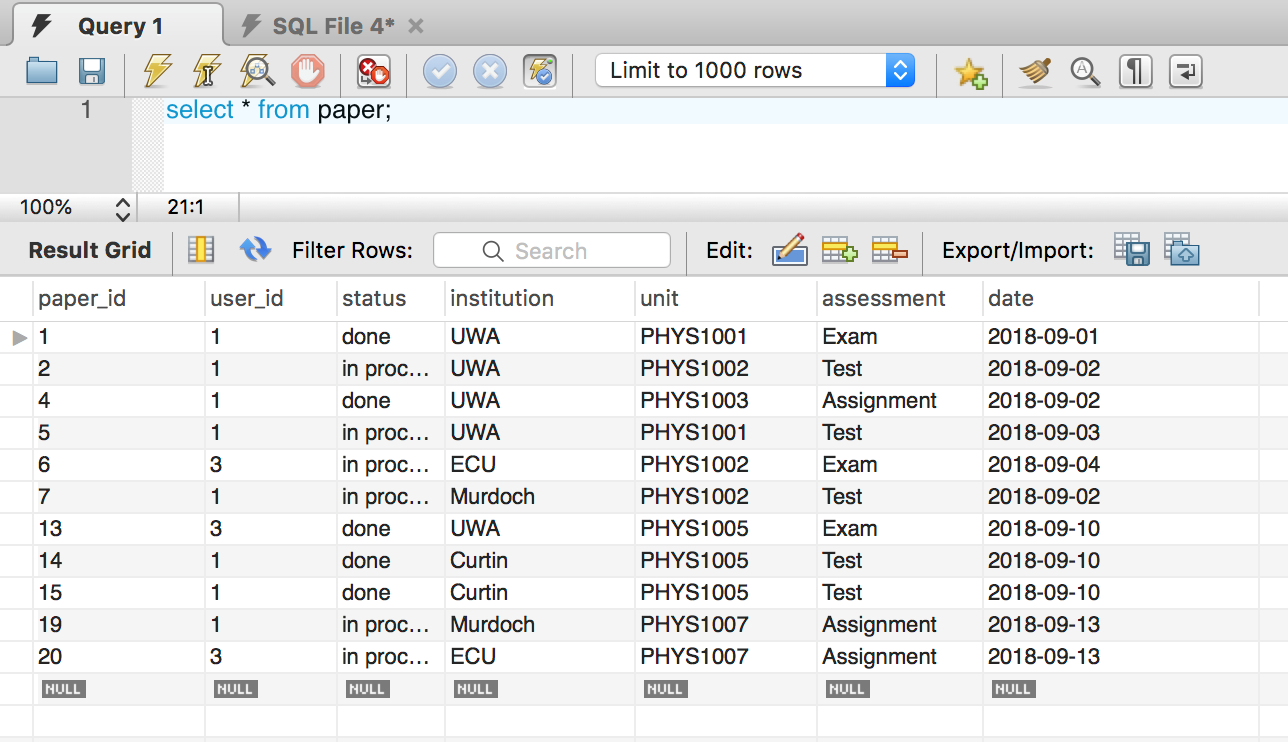
\includegraphics[width=8cm, height = 7cm]{newpaptable.PNG} }}%
    \qquad
    \subfloat[New In-Progress Paper Table]{{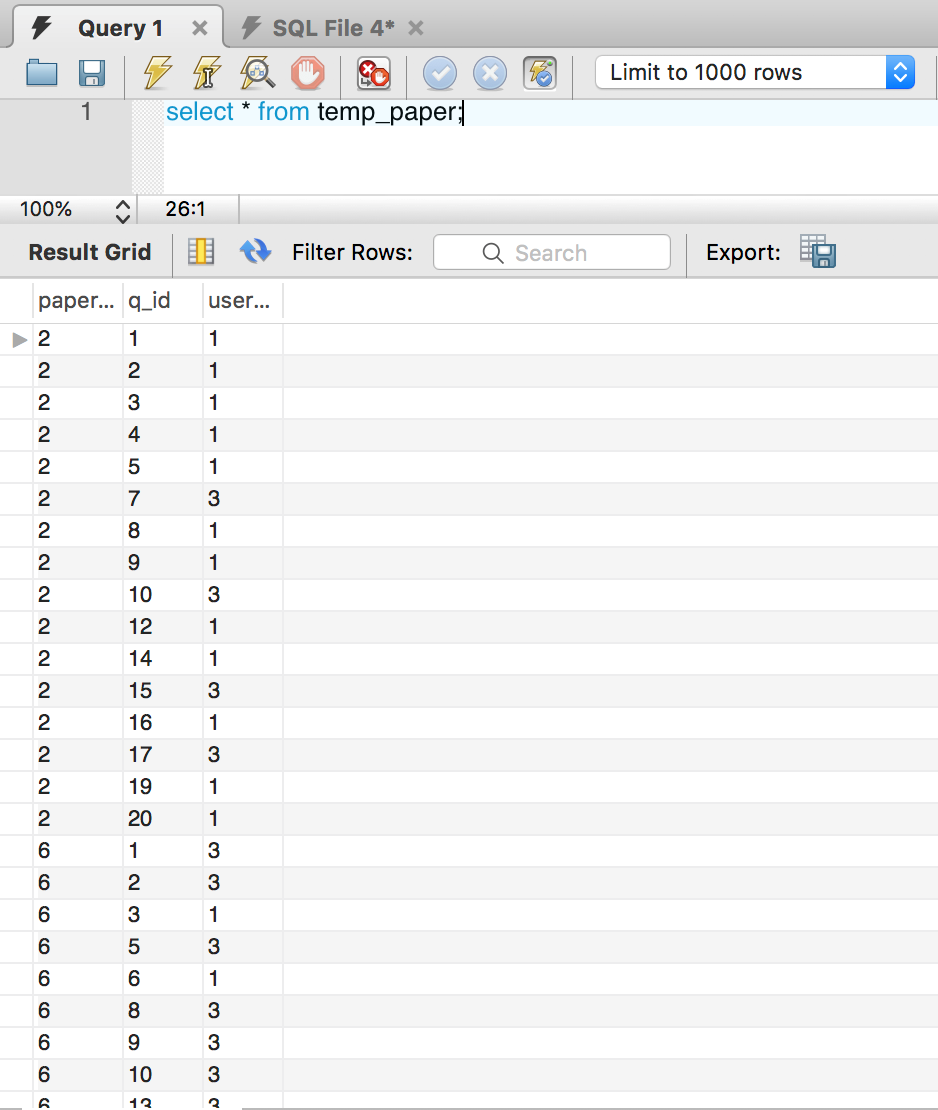
\includegraphics[width=6cm, height =8cm]{newtemptable.PNG} }}%
    \qquad
    \caption{Paper and In-Progress Paper Tables After User Deletion}
 \end{figure}

\chapter{Other General Notices, Warnings, and Errors}
\begin{table}[H]
\centering
\begin{tabular}{p{6cm} p{10 cm}}
\hline \hline
 Phenomenon & Explanation \\ \hline
 \normalsize 
 Cannot find the function to add a user to the System & Only the adminstrator of the whole system can add users to the application at this stage.\\\\
 Uploading Non-Zip Question Causes Crash & Ensure the format of the file you uploaded was of the type .zip, the system is designed to fault if there is a wrong file-type uploaded\\\\
 Uploading JPG or PDF as Preview Causes Crash & Ensure the format of the file you uploaded was of the type .png, the system is designed to fault if there is a wrong file-type uploaded\\\\
 Downloading a test and cancelled but now the test is gone & If you read the instructions carefully we warned against this since presently the database is updated \textbf{immediately }following the click of the download button to clean up after itself.\\\\
 \hline \hline
\end{tabular}
 \end{table}
\end{appendices}
\normalsize
\listoffigures

\end{document}
